% This is samplepaper.tex, a sample chapter demonstrating the
% LLNCS macro package for Springer Computer Science proceedings;
% Version 2.20 of 2017/10/04
%
\RequirePackage{amsmath}
\documentclass[runningheads]{llncs}
%
%This is a template for producing LIPIcs articles. 
%See lipics-manual.pdf for further information.
%for A4 paper format use option "a4paper", for US-letter use option "letterpaper"
%for british hyphenation rules use option "UKenglish", for american hyphenation rules use option "USenglish"
%for section-numbered lemmas etc., use "numberwithinsect"
%for enabling cleveref support, use "cleveref"
%for enabling cleveref support, use "autoref"


% \bibliographystyle{plainurl}% the mandatory bibstyle

\usepackage{graphicx}
\usepackage{algorithm}
\usepackage[noend]{algpseudocode}
\usepackage{amsmath}
\usepackage{amssymb}
% \usepackage{amsthm}
\usepackage{mathtools}
\usepackage{latexsym}
\usepackage{amstext}
\usepackage{xspace}
\usepackage{enumerate}
\usepackage{macrosLLNCS}
\usepackage{graphicx}
\usepackage{color}
\usepackage{epstopdf}
\usepackage{hyperref}
\hypersetup{
    colorlinks=true,
    linkcolor=black,
    filecolor=black,      
    urlcolor=blue,
    citecolor=black
}
% New definitions

\def\leaveout#1{}
\def\>{\ensuremath{\rangle}}
\def\<{\ensuremath{\langle}}
\def\h{\ensuremath{\mathcal{H}}}
\def\p{\ensuremath{\mathcal{P}}}
\def\l{\ensuremath{\mathcal{L}}}
\def\g{\ensuremath{\mathcal{G}}}
\def\lh{\ensuremath{\mathcal{L(H)}}}
\def\dh{\ensuremath{\mathcal{D(H})}}

\def\r{\ensuremath{\mathcal{R}}}

\def\ra{\ensuremath{\rightarrow}}
\def\e{\ensuremath{\mathcal{E}}}
\def\f{\ensuremath{\mathcal{F}}}

\def\c{\ensuremath{\mathcal{C}}}
\def\d{\ensuremath{\mathcal{D}}}
\def\le{\ensuremath{\sqsubseteq}}
\def\z{\ensuremath{{\bf 0}}}

\newcommand{\abis}{\stackrel{\lambda}\approx}
\newcommand{\abisa}[1]{\stackrel{#1}\approx}
\newcommand {\qbit} {\mbox{\bf{new}}}
\newcommand {\nil} {\mbox{\bf{nil}}}
\newcommand {\iif} {\mbox{\bf{if}}}
\newcommand {\then} {\mbox{\bf{then}}}
\newcommand {\eelse} {\mbox{\bf{else}}}
\newcommand {\qcf}[1] {{\sf{#1}}}
\newcommand{\con}[3]{\iif\ {#1}\ \then\ {#2}\ \eelse\ {#3}}

\newcommand{\ptr}{{\rm env}}
\newcommand{\rto}[1]{\stackrel{#1}\longrightarrow}
\newcommand{\Rto}[1]{\stackrel{#1}\Longrightarrow}
\newcommand{\nrto}[1]{\stackrel{#1}\nrightarrow}

\newcommand{\Rhto}[1]{\stackrel{\widehat{#1}}\Longrightarrow}
\newcommand{\define}{\stackrel{\it def}=}
\newcommand{\rsim}{\simeq}
\newcommand{\obis}{\approx_o}
%%%%%%%%%%%%%%%%% Distributions
\newcommand{\eDis}{\varepsilon}
\newcommand{\Stop}{{\times}}
\newcommand{\Mass}[1]{|#1|}
\newcommand{\subdist}[1]{\mathop{\mbox{$\mathcal D_{\textsl{sub}}$}}(#1)}
\newcommand{\dist}[1]{\mathop{Dist} ({#1})   } % distributions
\newcommand{\pdist}[1]{\overline{#1}  } % distributions
\newcommand{\support}[1]{\lceil{#1}\rceil}
\newcommand{\lift}[1]{\mathrel{{#1}^\circ}}

%%%%%%%%%%%%%%%% language
\newcommand{\probc}[1]{\mathrel{\!_{\scriptscriptstyle #1}\oplus}}
\newcommand{\Act}{\ensuremath{\mathsf{Act}}\xspace}

\newcommand{\setof}[2]{\{ \, #1 \, \mid \, #2 \, \}}% set comprehension
\newcommand{\Nat}{\mathbb{N}}
\newcommand{\Real}{\mathbb{R}}
\newcommand{\pair}[1]{\langle{#1}\rangle}
\newcommand{\ket}[1]{|{#1}\rangle}
\newcommand{\bra}[1]{\langle{#1}|}

%\newcommand{\so}{{\cal TSO}}
\newcommand{\Con}{{\it Con}}
\newcommand{\qv}{{\it qv}}
\newcommand{\qc}{\underline{c}}
\newcommand{\qd}{\underline{d}}
\newcommand{\cVar}{{\it cVar}}
\newcommand{\qVar}{{\it qVar}}
\newcommand{\cChan}{{\it cChan}}
\newcommand{\qChan}{{\it qChan}}
\newcommand{\tr}{{\rm tr}}
\newcommand{\CE}{{\cal E}}
\newcommand{\CH}{{\cal H}}
\newcommand{\CL}{{\cal L}}
\newcommand{\CC}{{\cal C}}
\newcommand{\CD}{{\cal D}}
\newcommand{\ifthen}[2]{{\textbf{if} ~#1~ \textbf{then} ~#2}}

\algnewcommand\algorithmicswitch{\textbf{switch}}
\algnewcommand\algorithmiccase{\textbf{case}}
\algnewcommand\algorithmicotherwise{\textbf{otherwise}}
\algnewcommand\algorithmicassert{\texttt{assert}}
\algnewcommand\Assert[1]{\State \algorithmicassert(#1)}%
% New "environments"
\algdef{SE}[SWITCH]{Switch}{EndSwitch}[1]{\algorithmicswitch\ #1\ \algorithmicdo}{\algorithmicend\ \algorithmicswitch}%
\algdef{SE}[CASE]{Case}{EndCase}[1]{\algorithmiccase\ #1}{\algorithmicend\ \algorithmiccase}%
\algdef{SE}[CASE]{Otherwise}{EndOtherwise}[1]{\algorithmicotherwise\ #1}{\algorithmicend\ \algorithmicotherwise}%
\algtext*{EndSwitch}%
\algtext*{EndCase}%
\algtext*{EndOtherwise}%
\usepackage{tabularx}
\usepackage{array}
\newcommand{\tabincell}[2]{\begin{tabular}{@{}#1@{}}#2\end{tabular}}

% New "environments"
\algdef{SE}[SWITCH]{Switch}{EndSwitch}[1]{\algorithmicswitch\ #1\ \algorithmicdo}{\algorithmicend\ \algorithmicswitch}%
\algdef{SE}[CASE]{Case}{EndCase}[1]{\algorithmiccase\ #1}{\algorithmicend\ \algorithmiccase}%
\algdef{SE}[CASE]{Otherwise}{EndOtherwise}[1]{\algorithmicotherwise\ #1}{\algorithmicend\ \algorithmicotherwise}%
\algtext*{EndSwitch}%
\algtext*{EndCase}%
\algtext*{EndOtherwise}%
\usepackage{tabularx}
\usepackage{array}
%\newcommand{\tabincell}[2]{\begin{tabular}{@{}#1@{}}#2\end{tabular}}

\makeatletter
\newenvironment{breakablealgorithm}
  {% \begin{breakablealgorithm}
   \begin{center}
     \refstepcounter{algorithm}% New algorithm
     \hrule height.8pt depth0pt \kern2pt% \@fs@pre for \@fs@ruled
     \renewcommand{\caption}[2][\relax]{% Make a new \caption
       {\raggedright\textbf{\ALG@name~\thealgorithm} ##2\par}%
       \ifx\relax##1\relax % #1 is \relax
         \addcontentsline{loa}{algorithm}{\protect\numberline{\thealgorithm}##2}%
       \else % #1 is not \relax
         \addcontentsline{loa}{algorithm}{\protect\numberline{\thealgorithm}##1}%
       \fi
       \kern2pt\hrule\kern2pt
     }
  }{% \end{breakablealgorithm}
     \kern2pt\hrule\relax% \@fs@post for \@fs@ruled
   \end{center}
  }
\makeatother

% Long table
\usepackage{longtable}
\usepackage{multirow}








% Used for displaying a sample figure. If possible, figure files should
% be included in EPS format.
%
% If you use the hyperref package, please uncomment the following line
% to display URLs in blue roman font according to Springer's eBook style:
% \renewcommand\UrlFont{\color{blue}\rmfamily}

\begin{document}
%
\title{Verifying Quantum Communication Protocols with Ground Bisimulation}
%
%\titlerunning{Abbreviated paper title}
% If the paper title is too long for the running head, you can set
% an abbreviated paper title here
%
\author{Xudong Qin\inst{1} \and
Yuxin Deng\inst{1}}
%
\authorrunning{X. Qin \and
Y. Deng}
% First names are abbreviated in the running head.
% If there are more than two authors, 'et al.' is used.
%
\institute{Shanghai Key Laboratory of Trustworthy Computing,\\ East China Normal University, China\\ \email{52174501019@stu.ecnu.edu.cn, yxdeng@sei.ecnu.edu.cn}}
%
\maketitle              % typeset the header of the contribution
%
\begin{abstract}
	
One important application of quantum process algebras is to formally verify quantum communication protocols. With a suitable notion of behavioural equivalence and a decision method, one can determine if an implementation of a protocol is consistent with the specification. Ground bisimulation is a convenient behavioural equivalence for quantum processes because of its associated coinduction proof technique. We exploit this technique to design and implement an on-the-fly algorithm to check if two given processes in quantum CCS are equivalent, which enables us to develop a tool that can verify interesting quantum protocols such as the BB84 quantum key distribution scheme.

\keywords{Quantum process algebra \and Bisimulation \and
Verification \and Quantum communication protocols.}
\end{abstract}
%
%
%
\section{Introduction}
\label{sec:introduction}
Process algebras provide a useful formal method for specifying and verifying concurrent systems. Their extensions to the quantum setting have also appeared in the literature. For example, Jorrand and Lalire \cite{JL04,La06} defined the \emph{Quantum Process Algebra} (QPAlg) and presented a branching bisimulation to identify quantum processes with the same branching structure. Gay and Nagarajan~\cite{GN05} developed \emph{Communicating Quantum Processes} (CQP), for which Davidson~\cite{Da11} established a bisimulation congruence.
Feng et al. \cite{FDJY07} have proposed a quantum variant of Milner's CCS \cite{ccs}, called qCCS, and a notion of probabilistic bisimulation for quantum processes, which is then improved to be a general notion of bisimulation that enjoys a congruence property \cite{FDY11}. Later on, motivated by~\cite{San96}, Deng and Feng~\cite{DF12} defined an open bisimulation for quantum processes that makes it possible to separate ground bisimulation and the closedness under super-operator applications, thus providing not only a neater and simpler definition, but also a new technique for proving bisimilarity.
In order to avoid the problem of instantiating quantum variables by potentially infinitely many quantum states, Feng et al. \cite{FDY14} extended the idea of symbolic bisimulation~\cite{HL95} for value-passing CCS and provided a symbolic version of open bisimulation for qCCS. They also proposed an algorithm for checking symbolic ground bisimulation.
 
In the current work, we consider the ground bisimulation proposed in \cite{DF12}. We put forward an on-the-fly algorithm to check if two given processes in qCCS with fixed initial quantum states are ground bisimilar. The algorithm is simpler than the one in \cite{FDY14} because the initial quantum states are determined for the former but can be parametric for the latter. Moreover, in many applications, we are only interested in the correctness of a quantum protocol with a predetermined input of quantum states. This is especially the case in the design stage of a protocol or in the debugging of a program. Meanwhile the algorithm can check the weak bisimulation where all internal actions are abstracted away by solving a linear programming problem.

The new algorithm is obtained by adapting the on-the-fly algorithm for checking probabilistic bisimulations \cite{Deng15}, which in turn has its root in similar algorithms
for checking classical bisimulations \cite{FM90,HL95}. The basic idea is as follows. A quantum process with an initial quantum state forms a configuration. We describe the operational behaviour of a configuration as a probabilistic labelled transition system (pLTS), where probabilistic transitions arise naturally because measuring a quantum system can entail a probability distribution of post-measurement quantum systems. The notion of ground bisimulation is a strengthening of probabilistic bisimulation by imposing some constraints on quantum variables and the environment states of processes. Therefore, the skeleton of the algorithm for quantum ground bisimulation resembles to that for probabilistic bisimulation.
We have developed a tool that can check if two given configurations are ground bisimilar. It is useful to validate whether an implementation of a protocol is equivalent to the specification. We have conducted experiments on a few interesting quantum protocols including super-dense coding, teleportation, secret sharing, and several quantum key distribution protocols, in particular the BB84 protocol~\cite{BB84}.

\paragraph{Other related work} 
 Ardeshir-Larijani et al. \cite{AL18} proposed a quantum variant of CCS to describe quantum protocols. The syntax of that variant is similar to qCCS but its semantics is very different. The behaviour of a concurrent process is a finite tree and an interleaving is a path from the root to a leaf. By interpreting an interleaving as a superoperator \cite{Sel04}, the semantics of a process is a set of superoperators. The equivalence checking between two processes boils down to the equivalence checking between superoperators, which is accomplished by using the stabiliser simulation algorithm invented by Aaronson and Gottesman~\cite{AG04}. Ardeshir-Larijani et al. have implemented their approach in an equivalence checker in Java and verified several quantum protocols from teleportation to secret sharing. 
However, they are not able to handle the BB84 quantum key distribution protocol because its correctness cannot be specified as an equivalence between interleavings.
Our approach is based on ground bisimulation and keeps all the branching behaviour of a concurrent process. Our algorithm for checking ground bisimulations is influenced by the on-the-fly algorithm of Hennessy and Lin for value-passing CCS \cite{HL95} and inspired by the probabilistic bisimulation checking algorithm of Baier et al. \cite{BEM00}.

Kubota et al. \cite{KKKKS16} implemented a semi-automated tool to check a notion of symbolic bisimulation and used it to verify the equivalence of BB84 and another quantum key distribution protocol based on entanglement distillation \cite{SP00}. There are two main differences between their work and ours. (1) Their tool is based on equational reasoning and thus requires a user to provide equations while our tool is fully automatic. (2) Their semantic interpretation of measurement is different and entails a kind of linear-time semantics for quantum processes that ignores the timepoints of the occurrences of probabilistic branches. However, we use a branching-time semantics. For instance, the occurrence of a measurement before or after a visible action is significant for our semantics but not for the semantics proposed in \cite{KKKKS16}.

Besides equivalence checking, based on either superoperators or bisimulations as mentioned above, model checking is another feasible approach to verify quantum protocols. For instance, Gay et al. developed the QMC model checker \cite{GNP08}.
Feng et al. implemented the tool QPMC \cite{FHTZ15} to model check quantum programs and protocols. There are also other approaches for verifying quantum systems. Abramsky and Coecke \cite{AC04} proposed a categorical semantics for quantum protocols. Quantomatic \cite{Kis11} is a semi-automated tool based on graph rewriting. Ying \cite{Yin16} established a quantum Hoare logic, which has been implemented in a theorem prover \cite{LLWYZ16}.

The rest of the paper is structured as follows. %In Sect.~\ref{sec:plts}, we introduce the formal model of probabilistic labelled transition systems. 
In Sect.~\ref{sec:qccs} we recall the syntax and semantics of the quantum process algebra qCCS. In Sect.~\ref{sec:algorithm} we present an algorithm for checking weak ground bisimulations. In Sect.~\ref{sec:experiment} we report the implementation of the algorithm and some experimental results on verifying a few quantum communication protocols. Finally, we conclude in Sect.~\ref{sec:con} and discuss some future work.


\section{Quantum CCS}\label{sec:qccs}

We introduce a quantum extension of classical CCS (qCCS) which was originally studied in \cite{FDJY07,YFDJ09,FDY11}. Three types of data are considered in qCCS: as classical data we have \texttt{Bool} for booleans and \texttt{Real} for real numbers, and as quantum data we have \texttt{Qbt} for qubits. Consequently,
two countably infinite sets of variables are assumed: $\cVar$ for classical variables, ranged over by $x,y,...$, and $\qVar$ for quantum variables, ranged over by $q,r,...$.
We assume a set ${\it Exp}$, which includes $\cVar$ as a subset and is ranged over by $e,e',\dots$,  of classical data expressions over
\texttt{Real}, and a set of boolean-valued expressions ${\it BExp}$, ranged over by $b, b',\dots$, with the usual boolean constants $\texttt{true}$, $\texttt{false}$, and operators
$\neg$, $\wedge$, $\vee$, and $\ra$. In particular, we let $e\bowtie e'$ be a boolean expression for any $e,e'\in {\it Exp}$ and ${\bowtie} \in\sset{>, <, \geq, \leq, =}$.
We further assume that only classical variables can occur freely in both data expressions and boolean expressions.
Two types of channels are used: $\cChan$ for classical channels, ranged over by $c,d,...$, and $\qChan$ for quantum channels, ranged over by $\qc,\qd$,.... A relabelling function $f$ is a map on $\cChan\; \cup\; \qChan$ such that $f(\cChan)\subseteq \cChan$ and $f(\qChan)\subseteq \qChan$.
Sometimes we abbreviate a sequence of distinct variables $q_1,...,q_n$ into $\tilde{q}$.

The terms in qCCS are given by:
\[\begin{array}{rcl}
P,Q &::=& \Cnil \BNFsep \tau.P \BNFsep c?x.P \BNFsep c!e.P
\BNFsep \qc?q.P \BNFsep
\qc!q.P \BNFsep \CE[\tilde{q}].P
\BNFsep M[\tilde{q};x].P \BNFsep \\
& & P + Q \BNFsep  P \Cpar Q\;
\BNFsep P[f] \BNFsep P\backslash L \BNFsep \ifthen{b}{P} \BNFsep
A(\tilde{q};\tilde{x})
\end{array}\]
where $f$ is a relabelling function and $L\subseteq \cChan\cup \qChan$ is a set of channels.
Most of the constructors are standard as in CCS \cite{ccs}.
We briefly explain a few new constructors. The process $\qc?q.P$ receives a quantum datum along quantum channel $\qc$ and evolves into $P$, while $\qc!q.P$ sends out a quantum datum along quantum channel $\qc$ before evolving into $P$. The symbol $\CE$ represents a trace-preserving super-operator applied on the systems $\tilde{q}$. The process $M[\tilde{q};x].P$ measures the state of qubits $\tilde{q}$
according to the observable $M$ and stores the measurement outcome into the
classical variable $x$ of $P$.

Free classical variables can be defined in the usual way, except for the fact that the variable $x$ in the quantum measurement $M[\tilde{q};x]$ is bound. A process $P$ is closed if it contains no free classical variable, i.e. $fv(P)=\emptyset$.

The set of free quantum variables for process $P$, denoted by $qv(P)$ can be inductively defined as in Figure~\ref{fig:fqv}.
\begin{figure*}[t]
	\[\small\begin{array}{rclrcl}
	qv(\Cnil) & = & \emptyset & qv(\tau.P) & = & qv(P)\\
	qv(c?x.P) & = & qv(P) & qv(c!e.P) & = & qv(P) \\
	qv(\qc?q.P) & = & qv(P)-\sset{q} & qv(\qc!q.P) & = & qv(P)\cup\sset{q} \\
	qv(\CE[\tilde{q}].P) & = & qv(P)\cup \tilde{q} &
	qv(M[\tilde{q};x].P) & = & qv(P) \cup \tilde{q}\\
	qv(P+Q) & = & qv(P)\cup qv(Q) \qquad &
	qv(P \Cpar Q) & = & qv(P)\cup qv(Q)\\
	qv(P[f]) & = & qv(P) &
	qv(P\backslash L) & = & qv(P)\\
	qv(\ifthen{b}{P}) & = & qv(P) &
	qv(A(\tilde{q};\tilde{x})) & = & \tilde{q}.
	\end{array}\]
	\caption{Free quantum variables}\label{fig:fqv}
\end{figure*}
For a process to be legal, we require that
\begin{enumerate}
	\item $q\not\in qv(P)$ in the process $\qc!q.P$;
	\item $qv(P)\cap qv(Q)=\emptyset$ in the process $P \Cpar Q$;
	\item Each constant $A(\tilde{q};\tilde{x})$ has a defining equation $A(\tilde{q};\tilde{x}) \Defs P$, where $P$ is a term with $qv(P)\subseteq\tilde{q}$ and $fv(P)\subseteq \tilde{x}$.
\end{enumerate}
The first condition says that a quantum system will not be referenced after it has been sent out. This is a requirement of the quantum no-cloning theorem. The second condition says that parallel composition $\Cpar$ models separate parties that never reference a quantum system simultaneously. 

\begin{figure*}[t]
	\[\small\begin{array}{ll}
	\slinfer[\Rlts{Tau}]{\pair{\tau.P, \rho} \ar{\tau} \pair{P, \rho}}
	&\linfer[\Rlts{C-Inp}]{v\in\texttt{Real}}{\pair{c?x.P,\rho} \ar{c?v} \pair{P[v/x],\rho}}
	\\[3pt]
	\linfer[\Rlts{C-Outp}]{v=\Op{e}}{\pair{c!e.P,\rho} \ar{c!v} \pair{P,\rho} }
	
	&
	\linfer[\Rlts{C-Com}]{\pair{P_1,\rho}\ar{c?v}\pair{P'_1,\rho}\qquad
		\pair{P_2,\rho}\ar{c!v}\pair{P'_2,\rho}
	}
	{\pair{P_1\Cpar P_2,\rho} \ar{\tau} \pair{P'_1\Cpar P'_2,\rho} }
	\\[3pt]
	\linfer[\Rlts{Q-inp}]{r\not\in qv(\qc?q.P)}
	{\pair{\qc?q.P,\rho} \ar{\qc?r} \pair{P[r/q],\rho}}
	&
	\slinfer[\Rlts{Q-Outp}]{\pair{\qc!q.P,\rho} \ar{\qc!q} \pair{P,\rho} }
	\\[3pt]
	\linfer[\Rlts{Q-Com}]{\pair{P_1,\rho} \ar{\qc?r} \pair{P'_1,\rho} \qquad \pair{P_2,\rho}\ar{\qc!r} \pair{P'_2,\rho}}
	{\pair{P_1\Cpar P_2, \rho } \ar{\tau} \pair{P'_1\Cpar P'_2, \rho}}
	&
	\slinfer[\Rlts{Oper}]{\pair{\CE[\tilde{q}].P,\rho} \ar{\tau} \pair{P,\CE_{\tilde{q}}(\rho)}}
	\\[3pt]
	\linfer[\Rlts{Meas}]{M=\sum_{i\in I}\lambda_i E^i \qquad p_i=tr(E^i_{\tilde{q}}\rho)}
	{\pair{M[\tilde{q};x].P,\rho} \ar{\tau} \sum_{i\in I}p_i \pair{P[\lambda_i/x], E^i_{\tilde{q}}\rho E^i_{\tilde{q}} / p_i}}
	&
	\\
	\linfer[\Rlts{Int}]{\pair{P_1,\rho} \ar{\alpha} \Delta\qquad qbv(\alpha)\cap qv(P_2)=\emptyset}{\pair{P_1 \Cpar P_2,\rho} \ar{\alpha} \Delta\Cpar P_2}
	%\\[3pt]
	%\linfer[\Rlts{Inp-Int}]{\pair{P_1,\rho} \ar{\qc?r} \pair{P'_1,\rho}\qquad r\not\in qv(P_2)}{\pair{P_1\Cpar P_2,\rho} \ar{\qc?r} \pair{P'_1\Cpar P_2,\rho}}
	&
	\linfer[\Rlts{Sum}]{\pair{P_1,\rho} \ar{\alpha} \Delta}{\pair{P_1+P_2,\rho} \ar{\alpha} \Delta}
	\\[3pt]
	\linfer[\Rlts{Rel}]{\pair{P,\rho} \ar{\alpha} \Delta}{\pair{P[f],\rho} \ar{f(\alpha)} \Delta[f]}
	&
	\linfer[\Rlts{Res}]{\pair{P,\rho} \ar{\alpha} \Delta \qquad cn(\alpha)\cap L=\emptyset}{\pair{P\backslash L,\rho} \ar{\alpha} \Delta\backslash L}
	\\[3pt]
	\linfer[\Rlts{Cho}]{\pair{P,\rho} \ar{\alpha} \Delta \qquad \Op{b}=\texttt{true}}{\pair{\ifthen{b}{P},\rho} \ar{\alpha} \Delta}
	&
	\linfer[\Rlts{Cons}]{\pair{P[\tilde{v}/\tilde{x},\tilde{r}/\tilde{q}],\rho} \ar{\alpha} \Delta \qquad A(\widetilde{x}, \tilde{q})\Defs P}{\pair{A(\tilde{v},\tilde{r}),\rho} \ar{\alpha} \Delta}
	\end{array}\]
	\caption{Operational semantics of qCCS. Here in rule $\Rlts{C-Outp}$, $\Op{e}$ is the evaluation of $e$, and in rule $\Rlts{Meas}$, $E^i_{\tilde{q}}$ denotes the operator $E^i$ acting on the quantum systems $\tilde{q}$.\label{fig:opsem}
	}
\end{figure*}

Throughout the paper we implicitly assume the convention that processes are identified up to $\alpha$-conversion, bound variables differ from each other and they are different from free variables.

Before introducing the operational semantics of qCCS processes, we review the model of probabilistic labelled
transition systems (pLTSs). Later on we will interpret the behaviour
of quantum processes in terms of pLTSs because quantum measurements give rise to probability distributions naturally.

We begin with some notations. A (discrete) probability distribution
over a set $S$ is a function $\Delta \colon S \rightarrow [0, 1] $ with
$\sum_{s\in S} \Delta(s) = 1$; the support of such a $\Delta$ is
the set $\support{\Delta} = \setof{s \in S}{\Delta(s) > 0}$.
The point distribution $\pdist{s}$ assigns probability
$1$ to $s$ and $0$ to all other elements of $S$, so that
$\support{\pdist{s}} = \{s\}$. We only need to use distributions with finite supports, and let $\dist{S}$ denote the set of
finite support distributions over $S$, ranged over by $\Delta$, $\Theta$, etc.
If $\sum_{k \in K} p_k = 1$ for some
collection of  $p_k \geq 0$, and the $\Delta_k$ are distributions,
then so is $\sum_{k \in K}p_k \cdot \Delta_k$ with
$(\sum_{k \in K}p_k \cdot \Delta_k)(s)~=~\sum_{k\in K} p_k\cdot \Delta_k(s).$


\begin{definition}\label{def:LTS}
	A \emph{probabilistic labelled transition system}
	is a triple
	$\langle S, \Act,  \rightarrow  \rangle$, where
	$S$ is a set of states,
	$\Act$ is a set of actions, and $\mathord{\rightarrow} \subseteq
	S \times \Act \times \dist{S}$ is the transition relation.
\end{definition}

We often write $s\ar{\alpha}\Delta$ for $(s,\alpha,\Delta)\in\mathord{\rightarrow}$. %, and $s\ar{\alpha}$ for $\exists \Delta: s\ar{\alpha}\Delta$.
In pLTSs we not only consider relations between states, but also relations between distributions. Therefore, we make use of the lifting operation below \cite{Deng15}.
\begin{definition}\label{def:lift}
	Let $\mathord{\aRel} \subseteq
	S\times S$ be a relation between states.
	Then $\mathord{\lift{\aRel}} \subseteq \dist{S} \times
	\dist{S}$ is the smallest relation that satisfies the two rules:
	(i) $s \aRel s'$ implies $\pdist{s} \lift{\aRel} \pdist{s'}$;
	(ii) $\Delta_i \lift{\aRel} \Theta_i$ for all $i\in I$ implies
	$(\sum_{i\in I}p_i\cdot\Delta_i)\lift{\aRel}(\sum_{i\in I}p_i\cdot\Theta_i)$
	for any $p_i \in [0,1]$ with $\sum_{i\in I}p_i = 1$, where $I$ is a
	finite index set.
\end{definition}

We now give the %turn to the %operational 
semantics of qCCS. For each quantum variable $q$ we assume a 2-dimensional Hilbert space $\CH_q$. For any nonempty subset $S\subseteq \qVar$ we write $\CH_S$ for the tensor product space $\bigotimes_{q\in S}\CH_q$ and $\CH_{\overline{S}}$ for $\bigotimes_{q\not\in S}\CH_q$. In particular, $\CH=\CH_{\qVar}$ is the state space of the whole environment consisting of all the quantum variables, which is a countably infinite dimensional Hilbert space.


Let $P$ be a closed quantum process and $\rho$ a density operator on $\CH$\footnote{As $\CH$ is infinite dimensional, $\rho$ should be understood as a density operator on some finite dimensional subspace of $\CH$ which contains $\h_{\qv(P)}$.}, the pair $\pair{P,\rho}$ is called a \emph{configuration}. We write $\Con$ for the set of all configurations, ranged over by $\CC$ and $\CD$.
We interpret qCCS with a pLTS whose states are all the configurations definable in the language,
and whose transitions are determined by the rules in Figure~\ref{fig:opsem}; we have omitted the obvious
symmetric counterparts to the rules \Rlts{C-Com}, \Rlts{Q-Com}, \Rlts{Int} and
\Rlts{Sum}.
The set of actions $\Act$ takes the following form, consisting of classical/quantum input/output actions.
\begin{eqnarray*}
\Act = 
	\sset{c?v, c!v \mid c\in \cChan, v\in\texttt{Real}}&\cup&
	\sset{\qc?r,\qc!r \mid \qc\in \qChan,r\in \qVar}
\end{eqnarray*}
%The symbol $\tau$ denotes invisible actions. We write $\Act$ for $\Act\cup\sset{\tau}$, which is ranged over by $\alpha$.
We use $cn(\alpha)$ for the set of channel names in action $\alpha$. For example, we have $cn(\qc?x)=\sset{\qc}$ and $cn(\tau)=\emptyset$.

In the first eight rules in Figure~\ref{fig:opsem}, the targets of arrows are point distributions, and we use the slightly abbreviated form $\CC\ar{\alpha}\CC'$ to mean $\CC\ar{\alpha}\pdist{\CC'}$.

The rules use the obvious extension of the function~$\Cpar$ on terms to configurations and distributions. To be precise,
$\CC\Cpar P$ is the configuration $\<Q\Cpar P,\rho \>$ where $\CC=\<Q,\rho\>$, and
$\Delta\Cpar P$ is the distribution defined by:
%\vskip -2mm
\[(\Delta\Cpar P)(\pair{Q,\rho}) \define \left\{\begin{array}{ll}
\Delta(\pair{Q',\rho}) & \mbox{if $Q=Q'\Cpar P$ for some } Q'\\
0 & \mbox{otherwise.}
\end{array}\right.\]
Similar extension applies to $\Delta[f]$ and $\Delta\backslash L$.

Suppose there is a configuration $\CC=\langle P,\rho\rangle$, the partial trace over system $P$ at such state can be defined as $tr_{qv(P)}(\rho)$. We give the definition of ground bisimulation and bisimilarity as follows. 
\begin{definition}[\cite{DF12}]\label{def:weak_bisim}
	A relation $\aRel\ \subseteq \Con\times\Con$ is a \emph{ground simulation} if
	$\CC\aRel \CD$ implies that $\qv(\CC)=\qv(\CD)$, $tr_{qv(P)}(\CC)=tr_{qv(Q)}(\CD)$,
	and
	\begin{itemize}
		\item whenever $\CC\ar{\alpha} \Delta$, there is some distribution $\Theta$ with $\CD\dar{\hat{\alpha}}_{c}\Theta$ and $\Delta \lift{\aRel} \Theta$.
	\end{itemize}
	A relation $\aRel$ is a \emph{ground bisimulation} if both $\aRel$ and
	$\aRel^{-1}$ are ground simulations. %Two configurations are \emph{ground bisimilar} if they are related by some ground bisimulation. 
	We denote by $\approx$ the largest ground bisimulation, called \emph{ground bisimilarity}.
\end{definition}

\section{Ground Bisimulation Checking Algorithm}\label{sec:algorithm}

In this section, we present an on-the-fly algorithm to check if two processes with fixed initial quantum configurations are ground bisimilar. For more detail, the algorithm updates two tables $NonBisim$ and $Bisim$ to record the verification results. $Bisim$ presents the ground bisimulation relation when the algorithm terminates. Furthermore, the algorithm returns $\texttt{true}$ if the initial configuration pair is contained in $Bisim$.

The decisive part of the algorithm is the check whether two configurations $t$ and $u$ are bisimilar. From  Definition~\ref{def:weak_bisim}, a pair of configurations is deemed non-bisimilar in three cases:
\vspace{-0.25em}
\begin{itemize}
    \item one configuration has a transition that cannot be matched by any possible weak combined transition from the other;
    \item they do not have the same set of free quantum variables for their processes;
    \item the density operators of them corresponding to their quantum registers are different.
\end{itemize}
\vspace{-0.25em}
The first case means that some actions of two configurations are not matched, that is, it violates the condition that if $t\overset{\alpha}{\longmapsto}\Delta$ then there exists some $u$ such that $u\overset{\alpha}{\mapstochar\Longrightarrow}_{c}\Theta$ and $\Delta \lift{\aRel} \Theta$. Here we use as a subroutine of the algorithm in \cite{TH15} to reduce the problem to a network flow problem that can be solved in polynomial time. The last two cases can be checked directly through the comparison of qubit sets and the computation of the trace of density operators.

Let $T$ be the set of transitions we may use when resolving the nondeterministic choices in a weak combined transition, $S$ be the set of states involved in these transitions, and $R$ be the equivalence relation of the states. We construct the flow network as follow.

Let $\vartriangle$ and $\blacktriangledown$ be two additional vertices represent the source and the sink of the network, respectively. The set of vertices $V$ is given below
\[V=\{\vartriangle,\blacktriangledown\}\cup S\cup S^{tr}\cup S_{\alpha}\cup S_{\alpha}^{tr}\cup S_{\bot}\cup S_{R}\] where
\begin{equation*}
    \begin{aligned}
    & S^{tr}=\{v^{tr}|tr=v \xmapsto{\beta} \rho ,\beta\in\{\alpha,\tau\}\};\\
    & S_{\alpha}=\{v_{\alpha}|v\in S\};\\
    & S_{\alpha}^{tr}=\{v_{\alpha}^{tr}|v^{tr}\in S^{tr}\};\\
    & S_{\bot}=\{v_{\bot}|v\in S\};\\
    & S_{R}=\{v_{R}|v\in S\}.
    \end{aligned}
\end{equation*}
and the set of edges $E$ is
\[E=\{(\vartriangle,s_{0})\}\cup L_{1}\cup L_{\alpha}\cup L_{2}\cup L_{\bot}^{\alpha}\cup L_{R}\] where
\begin{equation*}
    \begin{aligned}
    & L_{1}=\{(v,v^{tr}),(v^{tr},v')|tr=v\xmapsto{\tau}\rho\in T,v'\in\lceil\rho\rceil\};\\
    & L_{\alpha}=\{(v,v_{\alpha}^{tr}),(v_{\alpha}^{tr},v'_{\alpha})|tr=v\xmapsto{\alpha}\rho\in T,v'_{\alpha}\in\lceil\rho\rceil\};\\
    & L_{2}=\{(v_{\alpha},v_{\alpha}^{tr}),(v_{\alpha}^{tr},v'_{\alpha})|tr=v_{\alpha}\xmapsto{\tau}\rho\in T,v'_{\alpha}\in\lceil\rho\rceil\};\\
    & L_{\bot}^{\alpha}=\{(u_{
    \alpha},u_{\bot})|u\in S\};\\
    & L_{R}=\{(u_{\bot},v_{R}),(v_{R},\blacktriangledown)|(u,v)\in S_{R}\}.
    \end{aligned}
\end{equation*}

Given the transition $\mu\xmapsto{\alpha}\psi$, we check if the following linear programming problem has a solution.
\begin{flalign*}
    & max\sum\nolimits_{(u,v)\in E}-f_{u,v} &&\\
    s.t. & &&\\
    & f_{u,v}\ge0 && \text{for each }(u,v)\in E\\
    & f_{\vartriangle,s_0}=1 &&\\
    & f_{v_{R,\blacktriangledown}}=\psi(v) && \text{for each }v\in S\\
    & \sum\nolimits_{(u,v)\in E}f_{u,v}-\sum\nolimits_{(v,w)\in E}f_{v,w}=0 && \text{for each }v\in V\setminus\{\vartriangle,\blacktriangledown\}\\
    & f_{v^{tr},v'}-\rho(v')\cdot f_{v,v^{tr}}=0 && \text{for each }tr=v\xmapsto{\tau}\rho\in T\text{ and }v'\in\lceil\rho\rceil\\
    & f_{v_{\alpha}^{tr},v'_{\alpha}}-\rho(v'_{\alpha})\cdot f_{v,v_{\alpha}^{tr}}=0 && \text{for each }tr=v\xmapsto{\alpha}\rho\in T\text{ and }v'_{\alpha}\in\lceil\rho\rceil\\
    & f_{v_{\alpha}^{tr},v'_{\alpha}}-\rho(v'_{\alpha})\cdot f_{v_{\alpha},v_{\alpha}^{tr}}=0 && \text{for each }tr=v_{\alpha}\xmapsto{\tau}\rho\in T\text{ and }v'_{\alpha}\in\lceil\rho\rceil\\
\end{flalign*}

Intuitively, the fourth constraint is referred to as the flow-conservation constraints. The last three constraints link the source state and the result distribution. We introduce a predicate $\textbf{LP}(\psi,T,\alpha,R)$ which is true if and only if the linear programming problem has a solution.

\subsection{The Algorithm}
\label{sec:algorithm_code}
The function $\textbf{Bisim}(t,u)$, as what shown in Algorithm~\ref{alg:weak_bisim}, is the main function of the algorithm, which attempts to find the smallest bisimulation containing the pair $(t,u)$. It initialises $Bisim$ and a set named $Visited$ to store the visited pairs, then calls the function $\textbf{Match}$ with the initial configuration pair $(t,u)$ to search for a bisimulation. The function \textbf{Match}$(t,u,Visited)$ invokes a depth-first traversal to match a pair of configurations $(t,u)$ with all their possible behaviours. It checks whether the configuration pair encounters one of the three cases depicted before (Line 12-16). The set $Visited$ is updated before the traversal. This set is used for detecting loops. We match the behaviours of $t$ and $u$ from both directions as we are checking bisimulations.

An auxiliary function \textbf{Act}$(t)$ is invoked in \textbf{Match} to discover the next action that $t$ can perform as the parameter for the function \textbf{MatchAction}. If $t$ has no more action to do, the function will return an empty set.

Having defined the predicate \textbf{LP} before, we can defined the function $\textbf{MatchA}\\\text{-}\textbf{ction}(\alpha, t, u, Visited)$ to check whether the action of two configurations are matched. \textbf{MatchAction} invoke the function \textbf{Close}$(t,u,Visited)$ to construct an equivalence relation $R$ between the configurations from the target distribution and the weak transitions behaving the action asked.

To deal with loops, we update the set $Assumed$ to store all the assumptions we made. When the configuration pair to be considered is already contained in $Visited$ it will be assumed to be bisimilar and added to $Assumed$ (Line 42-44). Later on, if the pair of configurations are found to be non-bisimilar, it will be added to $NonBisim$ and a wrong assumption exception will be raised to restart the checking process from the original pair of configurations (Line 18-21). Then \textbf{Bisim}$(t, u)$ renews the set $Bisim$ and $Visited$ to remove the pairs checked under the wrong assumption (Line 8).

\begin{breakablealgorithm}
\caption{Checking ground bisimulation}
\label{alg:weak_bisim}
\begin{algorithmic}[1]
\Require Two pLTSs with  initial states $t$ and $u$.
\Ensure A boolean value $\theta$ indicating if the two pLTSs are ground bisimilar.
\Function{\textbf{GroundBisimulation}}{$t,u$} = 
\State $NonBisim$ := $\emptyset$
\State \textbf{function Bisim}($t, u$) = \textbf{try} \{
\State $Bisim$ := $\emptyset$
\State $Visited$ := $\emptyset$
\State $Assumed$ := $\emptyset$
\State \textbf{return} \textbf{Match}(\textit{t,u,Visited})
\State \} \textbf{catch WrongAssumptionException} $\Rightarrow$ \textbf{Bisim}($t, u$)
\EndFunction
\State
\Function{\textbf{Match}}{$t,u,Visited$}\Comment{$t=\langle P,\rho\rangle\ and\ u=\langle Q,\sigma\rangle$}
\State $Visited$:=$Visited\cup\{(t, u)\}$
\State $b$:=$\bigwedge_{\alpha\in \textit{Act}(t)}\textbf{MatchAction}(\textit{$\alpha$,t,u,Visited})$
\State $\overline{b}$:=$\bigwedge_{\alpha\in \textit{Act}(u)}\textbf{MatchAction}(\textit{$\alpha$,u,t,Visited})$
\State $b_{c_1}$:=$qv(P)=qv(Q)$
\State $b_{c_2}$:=$tr_{qv(P)}(\rho)=tr_{qv(P)}(\sigma)$
\State $b_{res}$:=$b\wedge\overline{b}\wedge b_{c_1}\wedge b_{c_2}$
\If{$b_{res}$ is \textbf{tt}} $Bisim=Bisim\cup\{(t,u)\}$
\ElsIf{$b_{res}$ is \textbf{ff}} 
    \State $NonBisim=NonBisim\cup\{(t,u)\}$
    \If{$(t,u)\in Assumed$} 
    \State \textbf{raise WrongAssumptionException} 
    \EndIf
\EndIf
\State \textbf{return} $b_{res}$ 
\EndFunction
\State
\Function{\textbf{MatchAction}}{$\alpha,t,u,Visited$}
\Switch{$\alpha$}
\Case{$c!$}
\For{$t\xrightarrow{c!e_i}\Delta_i$}
    \State Assume $\{t_{k}\}_{t_{k}\in \Delta_i}$ and $\{u_{j}\}_{u\xRightarrow{c!e'_j}u_{j}\wedge e_i=e'_j}$
    \State $R:=\{(t_k, u_j)|\textbf{Close}(t_k, u_j, Visited)=\textbf{tt}\}$
    \State $\theta$:=$\textbf{LP}(\Delta_i, \{u\xRightarrow{c!e'_j}u_{j}\}_{j}, \alpha, R)$
\EndFor
\State \textbf{return} $\bigwedge_{i}\theta_{i}$
\EndCase
\Otherwise{}
\For{$t\xrightarrow{\alpha}\Delta_i$}
    \State Assume $\{t_{k}\}_{t_{k}\in \Delta_i}$ and $\{u_{j}\}_{u\xRightarrow{\alpha}u_{j}}$
    \State $R:=\{(t_k, u_j)|\textbf{Close}(t_k, u_j, Visited)=\textbf{tt}\}$
    \State $\theta$:=$\textbf{LP}(\Delta_i, \{u\xRightarrow{\alpha}u_{j}\}_{j}, \alpha, R)$
\EndFor
\State \textbf{return} $\bigwedge_{i}\theta_{i}$
\EndOtherwise
\EndSwitch
\EndFunction
\State
\Function{\textbf{Close}}{$t, u, Visited$}
\If{$(t, u)\in Bisim$} \textbf{return} \textbf{tt}
\ElsIf{$(t, u)\in NonBisim$} \textbf{return} \textbf{ff}
\ElsIf{$(t, u)\in Visited$}
\State $Assumed=Assumed\cup\{(t,u)\}$
\State \textbf{return} \textbf{tt}
\Else \ \textbf{return} \textbf{Match}($t, u, Visited$)
\EndIf
\EndFunction
\end{algorithmic}
\end{breakablealgorithm}



\subsection{Termination and Correctness}
\label{sec:properties}
The proof of the termination and correctness of the algorithm is stated in Theorem~\ref{thm:termination} and~\ref{thm:correctness}. It relies on the sets updated during the execution of the algorithm. 

\begin{theorem}[Termination]\label{thm:termination}
Given two configurations $t$ and $u$, the function \textbf{GroundBisimulation(t,u)} always terminates.
\end{theorem}
\begin{proof}
%So far there is no while-loop in the qCCS, that brings convenience to the proof of termination. 
The algorithm starts with the empty sets $NonBisim$ and $Bisim$. Each execution of \textbf{Bisim} renews the sets except $NonBisim$. So we focus on the change of $NonBisim$. For a pair of configurations, the next action to perform will be detected in \textbf{Match}. Then it invokes function \textbf{MatchAction} to find the next new pair of configurations and recursively call function \textbf{Match} to check them. Each configuration pair checked non-bisimilar in function \textbf{Match} is added into $NonBisim$. Meanwhile, if it is contained in the set $Assumed$, that is, the algorithm has made an assumption such pair is bisimilar, the algorithm restarts a new execution of \textbf{Bisim} to solve the wrong assumption. Let variable $k$ denote the number of executions of \textbf{Bisim}, and $NonBisim_{k}$ be the set $NonBisim$ at the end of $\textbf{Bisim}_{k}$. The function updates $NonBisim_{k}$ at least once before it raising an exception. Hence, it is easy to show by induction that $NonBisim_{k}\subset NonBisim_{k+1}$ for any $k\geq 0$ except the last execution of $\textbf{Bisim}$ where the equality may be attained. As the system we considered contains finite configurations, there exists some $n$ such that $\textbf{Bisim}_{n}$ is the last execution of $\textbf{Bisim}$.

In the execution of $\textbf{Bisim}_{n}$, as it is the last time $\textbf{Bisim}$ run, no more exceptions will be raised. Each time \textbf{Match} executes with $t$ and $u$ as its parameters, we add $(t,u)$ into $Visited$. Furthermore, if we reach a node with no more action, we only compare the quantum variables used and the state of quantum registers. The function \textbf{Close} will not invoke $\textbf{Match}$ again if it meets the pair visited before. Since the system is finite, there will be no more configuration pairs added into $Visited$ and then no more $\textbf{Match}$ invoked. After finalizing all $\textbf{Match}$, the whole algorithm terminates.
\qed
\end{proof}

\begin{theorem}[Correctness]\label{thm:correctness}
Given two configurations $t$ and $u$ from two pLTSs, \textbf{GroundBisimulation}$(t,u)$ returns $\texttt{true}$ if and only if they are ground bisimilar.
\end{theorem} 
\begin{proof}
Let $\textbf{Bisim}_{n}$ be the last execution of $\textbf{Bisim}$, and $NonBisim_{n}$, $Bisim_{n}$ be the table recording the checked state pairs at the end of $\textbf{Bisim}_{n}$. From the branching statement of \textbf{Match} (Line 17-21), since only the pair of configurations not visited can be checked in \textbf{Match}, we can ensure that $NonBisim_{n}\cap Bisim_{n}=\emptyset$.

Then we discuss the final return of the $\textbf{Bisim}_{n}$. If the return is $\texttt{false}$ then we can conclude $s\not\sim t$ directly. If the return is $\texttt{true}$ then there is $Bisim_{n} = Visited_{n} - NonBisim_{n}$. According to the cases return $\texttt{true}$ in the function \textbf{Close} (Line 40,42-44), for each pair $(t, u)\in Bisim_{n}$, it satisfies that $\forall\alpha\in Act(t), t\overset{\alpha}{\longmapsto}\Delta\text{ then there exists } u \text{ such that } u\overset{\alpha}{\mapstochar\Longrightarrow}_{c}\Theta$, we have $\forall t'\in\lceil\Delta\rceil$, $\exists u'\in\lceil\Theta\rceil$, $(t', u')\in Assumed_{n}\cup Bisim_{n}$ and vice versa. Furthermore, as the algorithm always adds pairs into $Assumed_{n}$, if it is detected contained in $Visited_{n}$, we can imply that $Assumed_{n}\subseteq Visited_{n}$. As there is no more wrong assumption detected in the execution of $\textbf{Bisim}_{n}$, then we have $Assumed_{n}\subseteq Bisim_{n}$ which implies that $Bisim_{n}=Assumed_{n}\cup Bisim_{n}$ and $(t', u')\in Bisim_{n}$. We also ensure that $(t, u)\in Bisim_{n}$ satisfies that $qv(P)=qv(Q)$ and $tr_{qv(P)}(\rho)=tr_{qv(Q)}(\sigma)$, where $t=\langle P,\rho\rangle$ and $u=\langle Q,\sigma\rangle$. This relies on the checking statement in $\textbf{Match}$ before adding the pair to $Bisim_{n}$. Then by Definition.~\ref{def:weak_bisim}, $Bisim_{n}$ constitutes a bisimulation relation containing the root configuration pair $(t, u)$.
\qed
\end{proof}

At the end of this section, we analyse the time complexity of the algorithm.

\begin{theorem}[Complexity]\label{thm:complexity}
Let the number of nodes reachable from $t$ and $u$ be n. The time complexity of function \textbf{GroundBisimulation}$(t,u)$ is polynomial in $n$. % and the space complexity of it is $O(n^2)$.
\end{theorem}
\begin{proof}
The number of state pairs is at most $n^2$. The number of state pairs examined in the $k$th execution of \textbf{Bisim} is at most $O(n^2-k)$. Therefore, the total number of state pairs examined is as most $O(n^2+(n^2-1)+...+1)=O(n^4)$. Since the pLTSs are assumed to be finite trees, the number of comparisons of transitions does not exceed some constant. Moreover, each comparison may call the function \textbf{LP} at most once, where constructing of the flow network and solving the linear programming problem are both polynomial in $n$ if we use the algorithm in~\cite{TH15}. 
% The time complexity of solving the linear programming problem is up to the method we choose such as two-phase simplex algorithm. 
As a result, the whole algorithm is also polynomial in $n$.
\qed
\end{proof}

\section{Implementation and Experiments}
\label{sec:experiment}
In this section, we report on an implementation of our approach and provide the experimental results of the verification of several quantum communication protocols. 

\begin{figure}[htbp]
\centering
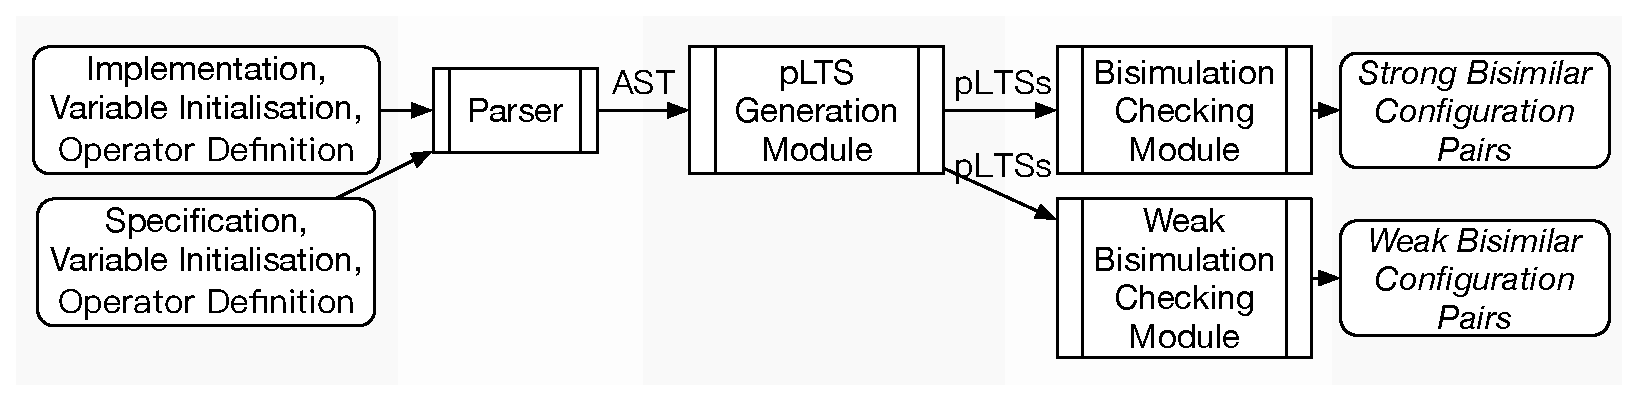
\includegraphics[width=\textwidth]{images/architecture.eps}
\caption{Verification workflow.}
\label{fig:arch}
\vspace{-1em}
\end{figure}

\subsection{Implementation}
We have implemented both strong and weak ground bisimulation checkers, written in Python 3.7. The algorithm for checking strong bisimulation is shown in Appendix~\ref{sec:strong_bisim}. The workflow of our tool is sketched in Figure~\ref{fig:arch}. The tool consists of a pLTS generation module and a bisimulation checking module, devoted to modeling and verification, respectively.
The tool inputs a specification and an implementation of a quantum protocol, both described as qCCS processes, the definition of user-defined operators (some of them are shown in Appendix~\ref{sec:appc}), as well as an initialisation of classical and quantum variables. Unlike classical variables, the initialisation of all quantum variables, deemed as a quantum register, is accomplished at the same time so to allow for superposition states.
The final output of the tool is a result indicating whether the specification and the implementation are bisimilar under the same initial configurations. The algorithm records the bisimilar pairs and non-bisimilar pairs, i.e., the bisimulation relation is figured out in the traversal of configuration pairs.
%
%\subparagraph*{pLTS Generation Module.}

The pLTS generation module acts as a preprocessing unit before the verification task. It first translates the input qCCS processes into two abstract syntax trees (ASTs) by a parser. Then the ASTs are transformed into two pLTSs according to the operational semantics given in Figure~\ref{fig:opsem}, using the user-defined operators and the initial values of variables.
%
%\subparagraph*{Bisimulation Checking Module.} 
The bisimulation checking module implements the ground weak bisimilarity checking algorithm we defined in the last section. It checks whether the initial states of the two generated pLTSs are weak bisimilar. 
%The execution result presents whether these two pLTSs are bisimilar attached with a set of non-bisimilar state pairs and a set of bisimilar state pairs.

The tool is available in \cite{QBisim},
where we also provide all the examples for the experiments to be discussed in Section~\ref{sec:exper}. %\url{https://github.com/MartianQXD/QBisim}. 
%It has already prepared codes of the examples we used in directories \textsl{examples}.

\subsection{BB84 Quantum Key Distribution Protocol}
\label{sec:bb84}
To illustrate the use of our tool,
we formalise the BB84 quantum key distribution protocol. Our formalisation follows \cite{DF12}, where a manual analysis of the protocol is provided. Now we perform automatic verification via the ground bisimulation checker.
More examples are given in Appendix~\ref{sec:examples}.
% Now we perform automatic verification via the strong ground bisimulation checker.

%We display four examples in our experiment: (1) super-dense coding protocol; (2) quantum teleportation protocol; (3) quantum secret sharing; (4) BB84 quantum key kistribution protocol. Below we make a brief introduction to the quantum secret sharing protocol as an illustration. Other examples are given in Appendix~\ref{sec:examples}.

The BB84 protocol provides a provably secure way to create a private key between two partners with a classical authenticated channel and a quantum insecure
channel between them. The protocol does not make use of entangled states. It ensures its security through the basic property of quantum mechanics: if the states to be distinguished are not orthogonal, such as $|0\rangle$ and $|+\rangle$, then information gain about a quantum state is only possible at the expense of changing the state. Let the sender and the receiver be $Alice$ and $Bob$, respectively. The basic BB84 protocol with a sequence of qubits $\tilde{q}$ with size $n$ goes as follows:
\begin{enumerate}
	\item $Alice$ randomly generates two sequences of bits $\tilde{B}_a$ and $\tilde{K}_a$ using her qubits $\tilde{q}$. Note that $\tilde{q}$ here are auxiliary qubits for random generation which are not modified in this step.
	\item $Alice$ sets the state of $\tilde{q}$, such that the \textit{i}th bits of $\tilde{q}$ is $|x_{y}\rangle$ where $x$ and $y$ are the \textit{i}th bits of $\tilde{B}_a$ and $\tilde{K}_a$, and respectively, $|0_0\rangle=|0\rangle$, $|0_1\rangle=|1\rangle$, $|1_0\rangle=|+\rangle=(|0\rangle+|1\rangle)/\sqrt{2}$ and $|1_1\rangle=|-\rangle=(|0\rangle-|1\rangle)/\sqrt{2}$.
	\item $Alice$ sends her qubits $\tilde{q}$ to $Bob$.
	\item $Bob$ randomly generates a sequence of bits $\tilde{B}_b$ using his qubits $\tilde{q}'$.
	\item $Bob$ measures the \textit{i}th qubit of $\tilde{q}$ he received from $Alice$ according to the basis determined by the \textit{i}th bit of $\tilde{B}_b$. Respectively, the basis is $\{|0\rangle,|1\rangle\}$ if it is $0$ and $\{|+\rangle,|-\rangle\}$ if it is $1$.
	\item $Bob$ sends his choice of measurements $\tilde{B}_{b}$ to $Alice$, and after receiving the information, $Alice$ sends her $\tilde{B}_{a}$ to $Bob$.
	\item $Alice$ and $Bob$ match two sequences of bits $\tilde{B}_{a}$ and $\tilde{B}_{b}$ to determine at which positions the bits are equal. If the bits match, they keep the corresponding bits of $\tilde{K}_a$ and $\tilde{K}_b$. Otherwise, they discard them.
\end{enumerate}
After the execution of the basic BB84 protocol, the remaining bits of $\tilde{K}_a$ and $\tilde{K}_b$ should be the same, provided that the communication channels are perfect and there is no eavesdropper.

Then we consider the case that there exists an eavesdropper called $Eve$ taking part in the communication. $Alice$ and $Bob$ also have more behaviours to detect $Eve$. In the BB84 protocol with an eavesdropper, let $\tilde{K'}_a$ and $\tilde{K'}_b$ to be the remaining bits of $\tilde{K}_a$ and $\tilde{K}_b$ with size $k$. Then $Alice$, $Bob$ and $Eve$ proceed as follows:
\begin{enumerate}
	\item $Alice$ randomly chooses $\lceil k/2\rceil$ bits of $\tilde{K'}_a$, denoted by $\tilde{K''}_a$ and sends it to $Bob$ together with the indexes of the chosen bits.
	\item After receiving the information from $Alice$, $Bob$ chooses $\lceil k/2\rceil$ bits of $\tilde{K'}_b$ according to the indexes he received, denoted by $\tilde{K''}_b$ and sends it back to $Alice$.
	\item $Alice$ and $Bob$ match two sequences of bits $\tilde{K''}_{a}$ and $\tilde{K''}_{b}$. If the two sequences match, then they have not detected the eavesdropper and the remaining substrings of $\tilde{K'}_{a}$ and $\tilde{K'}_{b}$ are used as the secure key. Otherwise, they detect $Eve$ and the protocol halts without generating any secure keys.
\end{enumerate}

\paragraph{Implementation.}
For simplicity, we assume that the sequence $\tilde{q}$ consists of only one qubit. This is enough to reflect the essence of the protocol. The other qubits used below are auxiliary qubits for the operation $Ran$.
\begin{flalign*}
Alice \overset{def}{=}& Ran[q_1;B_{a}].Ran[q_1;K_{a}].Set_{K_{a}}[q_1].H_{B_{a}}[q_1].\underline{A2B}!q_1.\\ 
&\qquad\qquad\qquad b2a?B_{b}.a2b!B_{a}.key_{a}!cmp(K_{a},B_{a},B_{b}).\textbf{nil};\\
Bob \overset{def}{=}& \underline{A2B}?q_1.Ran[q_2;B_{b}].M_{B_{b}}[q_1;K_{b}].b2a!B_{b}.\\
&\qquad\qquad\qquad a2b?B_{a}.key_{b}!cmp(K_{b},B_{a},B_{b}).\textbf{nil};\\
BB84 \overset{def}{=}& (Alice||Bob)\setminus\{a2b,b2a,\underline{A2B}\}
\end{flalign*}
where there are several special operations:
\begin{itemize}
	\item $Ran[q;x]$ is equal to quantum operations $Set_{+}[q].M_{0,1}[q;x].Set_{0}[q]$, where $Set_{+}$ (resp.$Set_{0}$) is the operation which sets a qubit it applies on to $|+\rangle$ (resp.$|0\rangle$), $M_{0,1}[q;x]$ is the quantum measurement on $q$ according to the basis $\{|0\rangle,|1\rangle\}$ and stores the result into $x$.
	\item $Set_{K}[q]$ sets the qubit $q$ to the state $|K\rangle$.
	\item $H_{B}[q]$ applies $H$ or does nothing on the qubit $q$ depending on whether the value of $B$ is 1 or 0.
	\item $M_{B}[q;K]$ is the quantum measurement on $q$ according to the basis $\{|+\rangle,|-\rangle\}$ or $\{|0\rangle,|1\rangle\}$ depending on whether the value of $B$ is 1 or 0.
	\item $cmp(x,y,z)$ returns $x$ if $y$ and $z$ match, and $\epsilon$, meaning it is empty, if they do not match.
\end{itemize}
\paragraph{Specification.}
The specification can be defined as follows using the same operations:
\begin{flalign*}
BB84_{spec} \overset{def}{=}& Ran[q_1;B_{a}].Ran[q_1;K_{a}].Ran[q_2;B_{b}]\\
&\qquad\qquad.(key_{a}!cmp(K_{a},B_{a},B_{b}).\textbf{nil}||key_{b}!cmp(K_{a},B_{a},B_{b}).\textbf{nil}).
\end{flalign*}

\paragraph{Input.}
For the implementation of $BB84$, we need to declare the following variables and operators in the input attached to it.
\begin{itemize}
    \item The classical bits are named $B_a$, $K_a$ for $Alice$ and $B_b$, $K_b$ for $Bob$.
    \item The qubits are declared together as a vector $|q_1,q_2\rangle$. The vector always needs an initial value. We can set it to be $|00\rangle$ in this example.
\end{itemize}
When modelling the protocol, we use several operators. They should be defined and their definitions are part of the input. 
\begin{itemize}
    \item The operator $Ran$ involves two operators $Set_{+}$, $Set_{0}$ and a measurement $M_{0,1}$ measuring the qubit according to the basis $\{|0\rangle,|1\rangle\}$. 
    \item $Set_{K}$ needs $Set_{0}$ and $Set_{1}$.
    \item $H_{B}$ requires the Hadamard gate $H$.
    \item $M_{B}$ uses the measurement $M_{+,-}$ which measures the qubit according to the basis $\{|+\rangle,|-\rangle\}$. 
\end{itemize}
The function $cmp$ is treated as an in-built function, so there is no need to define it in the input.

For the specification $BB84_{spec}$, we only declare the classical bits $B_a$, $B_b$, $K_a$, qubits $q_1$, $q_2$ and the operator $Ran$. The variables and operators declared here are the same as those in the input of the implementation.

\paragraph{Output.}
Taking the input discussed above, the tool first generates two pLTSs, with over 150 states for the implementation and 80 states for the specification, and then runs the ground bisimulation checking algorithm. As we can see from the third last row in Table~\ref{tab:weak_result} in next section, our tool confirms that $\langle BB84, \rho_0\rangle \sim \langle BB84_{spec}, \rho_0\rangle$, where $\rho_0$ denotes the initial state of the quantum register, thus the implementation is faithful to the specification. In the output of the tool, there is an enumeration of 1084 pairs of non-bisimilar states and 3216 pairs of bisimilar states. The pLTSs and the state pairs can be found in \cite{QBisim}.

\paragraph{Implementation with an Eavesdropper.}
We proceed to model the protocol with an eavesdropper. For that purpose, we extend the processes $Alice$ and $Bob$ with two processes for eavesdropper detection.
\begin{flalign*}
% Alice' \overset{def}{=}& key_{a}?K'_{a}.Pstr_{|K'_{a}|}[q_1;x].a2b!x.a2b!SubStr(K'_{a},x).b2a?K''_{b}.\\
% &(\textbf{if}\ SubStr(K'_{a},x)=K''_{b}\ \textbf{then}\ key'_{a}!RemStr(K'_{a},x).\textbf{nil} \\
% & + \textbf{if not}\ \ SubStr(K'_{a},x)=K''_{b}\ \textbf{then}\  alarm_{a}!0.\textbf{nil});\\
% Bob' \overset{def}{=}& key_{b}?K'_{b}.a2b?x.a2b?K''_{a}.b2a!SubStr(K'_{b},x).\\
% &(\textbf{if}\ SubStr(K'_{b},x)=K''_{a}\ \textbf{then}\ key'_{b}!RemStr(K'_{b},x).\textbf{nil} \\
% & + \textbf{if not}\ \ SubStr(K'_{b},x)=K''_{a}\ \textbf{then}\  alarm_{b}!0.\textbf{nil})\\
Alice' \overset{def}{=}& key_{a}?K'_{a}.Pstr_{|K'_{a}|}[q_1;x].a2b!x.a2b!SubStr(K'_{a},x).b2a?K''_{b}.\\
&(\textbf{if}\ SubStr(K'_{a},x)=K''_{b}\ \textbf{then}\ key'_{a}!RemStr(K'_{a},x).\textbf{nil} \\
& + \textbf{if not}\ SubStr(K'_{a},x)=K''_{b}\ \textbf{then}\ msg_{a}!0.\textbf{nil});\\
Bob' \overset{def}{=}& key_{b}?K'_{b}.a2b?x.a2b?K''_{a}.b2a!SubStr(K'_{b},x).\\
&(\textbf{if}\ SubStr(K'_{b},x)=K''_{a}\ \textbf{then}\ key'_{b}!RemStr(K'_{b},x).\textbf{nil} \\
& + \textbf{if not}\ SubStr(K'_{b},x)=K''_{a}\ \textbf{then}\ msg_{b}!0.\textbf{nil})
\end{flalign*}
where there are three more special operations:
\begin{itemize}
	\item $Pstr_m$ is a measurement similar to $Ran$; it randomly generates a sequence of $\lceil m/2\rceil$ bits ranging from 1 to $m$. As there is only one bit in this example, here it just generates the value of $x$.
	\item $SubStr(K,x)$ returns the substring of $K$ at the index specified by $x$. As the example here only consider one bit, $x$ decides the return is $K$ or nothing.
	\item $RemStr(K,x)$ returns the remaining substring of $K$ deleting $SubStr(K,x)$.
\end{itemize}

Then we define the eavesdropper as follows.
\begin{flalign*}
Eve \overset{def}{=}& \underline{A2E}?q_1.Ran[q_3;B_{e}].M_{B_{e}}[q_1;K_{e}].Set_{K_{e}}[q_1].H_{B_{e}}[q_1].\underline{E2B}!q_1.key_{e}!K_{e}.\textbf{nil}.
\end{flalign*}
With the participation of $Eve$, we adjust the communication of $Alice$ and $Bob$:
\begin{flalign*}
Alice\rightarrow Alice[f_{a}],\qquad Bob\rightarrow Bob[f_{b}]
\end{flalign*}
where $f_{a}(\underline{A2B})=\underline{A2E}$, and $f_{b}(\underline{A2B})=\underline{E2B}$.

Next, we introduce a test process $Test$ before arriving at the new implementation $BB84'$:
\begin{flalign*}
% Test \overset{def}{=}& key'_{a}?x.key'_{b}?y.key'_{e}?z.\\
% &(\textbf{if}\ x\neq y\ \textbf{then}\  fail!0.\textbf{nil}\\
% &\ +\ \textbf{if}\ x=y\ \textbf{then}\ key_{e}!z.skey!x.\textbf{nil});\\
Test \overset{def}{=}& key'_{a}?x.key'_{b}?y.key'_{e}?z.\\
&\qquad(\textbf{if}\ x\neq y\ \textbf{then}\ fail!0.\textbf{nil}\ +\ \textbf{if}\ x=y\ \textbf{then}\ key_{e}!z.skey!x.\textbf{nil})\\
+&\ msg_{a}?x.msg_{b}?y.key'_{e}?z.alarm!0.\textbf{nil};\\
BB84' \overset{def}{=}& (Alice||Bob||Alice'||Bob'||Eve||Test)\setminus C
\end{flalign*}
where $C=\{a2b,b2a,key_{a},key_{b},\underline{A2E},\underline{E2B},alarm\}$.
\paragraph{Specification with an Eavesdropper.}
Taking into account the presence of an eavesdropper, we define the new specification as follows:
\begin{flalign*}
BB84'_{spec} \overset{def}{=}& Ran[q_1;B_{a}].Ran[q_1;K_{a}].Ran[q_3;B_{e}].Ran'_{B_{a},B_{e},K_{a}}[q_1;K_{e}].\\
&Ran[q_2;K_{b}].Ran'_{B_{e},B_{b},K_{e}}[q_1;K_{b}].Pstr_{K_{ab}}[q_1;x].\\
&(\textbf{if}\ K_{ab}=K_{ba}\ \textbf{then}\ key_{e}!K_{e}.skey!RemStr(K_{ab},x).\textbf{nil}\\
&\ + \textbf{if}\ K_{ab}\neq K_{ba}\ \textbf{then}\ (\textbf{if}\ K^{x}_{ab}\neq K^{x}_{ba}\ \textbf{then}\ alarm!0.\textbf{nil}\\
&\qquad\qquad\qquad\qquad\qquad\ + \textbf{if}\ K^{x}_{ab}=K^{x}_{ba}\ \textbf{then}\ fail!0.\textbf{nil}))
\end{flalign*}
where $K_{ab}=cmp(K_{a},B_{a},B_{b})$,  $K_{ba}=cmp(K_{b},B_{a},B_{b})$, $K^{x}_{ab}=SubStr(K_{ab},x)$, $K^{x}_{ab}=SubStr(K_{ba},x)$. And similar to $Ran$, $Ran'_{x,y,z}[q;v]$ is a special measurement that randomly generates the value of $v$ if $x$ and $y$ do not match and give $v$ the value of $z$ if they match.

%\subparagraph*{More Inputs.}
\smallskip
As to the input, we need to declare more variables for $BB84'$ as there are more roles involved in the communication.
\begin{itemize}
    \item The classical bits named $K'_a$, $K''_a$ for $Alice$ are used for storing the result of processing the sequence. The bits $K'_b$, $K''_b$ for $Bob$ do the same work.
    \item The classical bits for $Eve$ are named $B_e$ and $K_e$.
    \item The classical bits named $x$, $y$, $z$ are declared to store the remaining string.
    \item The qubits are declared together to be a longer vector $|q_1,q_2,q_3\rangle$. We set it to be $|000\rangle$ in this example.
\end{itemize}
Similar to the function $cmp$, the functions $SubStr$ and $RemStr$ are already declared inside the tool. 

For the specification $BB84'_{spec}$, we declare the bits $K_{ab}$, $K_{ba}$, $K^x_{ab}$ and $K^x_{ba}$. Certainly, we still need to declare $B_e$ and $K_e$.

% We see from the second last row in Table~\ref{tab:strong_result} that in this case our tool gives a negative verification result, i.e. $\langle BB84',\rho_0\rangle \not\sim \langle BB84'_{spec},\rho_0\rangle$. In other words, the implemention $BB84'$ is unsatisfactory. 
% After carefully examining the behaviour of the process $BB84'$, we find that the problem lies in the fact that $Alice'$ and $Bob'$ have excessive freedom to trigger alarms. 
% $Alice$ and $Bob$ will declare an alarm if their measurement methods are not matched. The parallelism between the final test process and them leads to a process that continues exhibiting undesirable actions. This is not what the specification exactly describes. The implementation has more behaviours than what the specification requires. 
% Some modification is needed to make it behave the same as the specification.

% \paragraph{Improved BB84 Protocol with an Eavesdropper.}

% We fix the problem discussed above by requiring $Alice'$ and $Bob'$ to communicate with $Test$ before the latter triggers an alarm, thus we move the delaration of alarms to the test process. $Alice'$ and $Bob'$ only send messages when  they use different measurements. 
% The following three processes are updated:
% \begin{flalign*}
% Alice' \overset{def}{=}& key_{a}?K'_{a}.Pstr_{|K'_{a}|}[q_1;x].a2b!x.a2b!SubStr(K'_{a},x).b2a?K''_{b}.\\
% &(\textbf{if}\ SubStr(K'_{a},x)=K''_{b}\ \textbf{then}\ key'_{a}!RemStr(K'_{a},x).\textbf{nil} \\
% & + \textbf{if not}\ SubStr(K'_{a},x)=K''_{b}\ \textbf{then}\ msg_{a}!0.\textbf{nil});\\
% Bob' \overset{def}{=}& key_{b}?K'_{b}.a2b?x.a2b?K''_{a}.b2a!SubStr(K'_{b},x).\\
% &(\textbf{if}\ SubStr(K'_{b},x)=K''_{a}\ \textbf{then}\ key'_{b}!RemStr(K'_{b},x).\textbf{nil} \\
% & + \textbf{if not}\ SubStr(K'_{b},x)=K''_{a}\ \textbf{then}\ msg_{b}!0.\textbf{nil});\\
% Test \overset{def}{=}& key'_{a}?x.key'_{b}?y.key'_{e}?z.\\
% &(\textbf{if}\ x\neq y\ \textbf{then}\  fail!0.\textbf{nil}\ +\ \textbf{if}\ x=y\ \textbf{then}\ key_{e}!z.skey!x.\textbf{nil})\\
% &+\ msg_{a}?x.msg_{b}?y.key'_{e}?z.alarm!0.\textbf{nil}.
% \end{flalign*}
% The last row in Table~\ref{tab:strong_result} tells us that the above modification of the implementation is indeed correct.

\subsection{Experimental Results}\label{sec:exper}
We conducted experiments on several quantum communication protocols with a few different input variables.  
Table~\ref{tab:weak_result} provides a summary of our experimental results obtained on a macOS machine with an Intel Core i7 2.5 GHz processor and 16GB of RAM.

\begin{table}[htbp]
\vspace{-1em}
\scriptsize
\centering
\begin{tabular}{@{}m{0pt}@{}
                >{\centering\arraybackslash}m{2.5cm}
                ||>{\centering\arraybackslash}m{4cm}
                |>{\centering\arraybackslash}m{0.6cm}
                |>{\centering\arraybackslash}m{0.6cm}
                |>{\centering\arraybackslash}m{0.6cm}
                |>{\centering\arraybackslash}m{0.6cm}
                |>{\centering\arraybackslash}m{0.6cm}
                |>{\centering\arraybackslash}m{1cm}}
\hline
\multicolumn{9}{c}{\textbf{Weak bisimulation}}\\
\hline
\hline
\rule{0pt}{3mm}&\textbf{Program} & \textbf{Variables} & \textbf{Bis} & \textbf{Imp} & \textbf{Spe} & \textbf{N} & \textbf{B} & \textbf{ms} \\
\hline
\hline
\rule{0pt}{3mm}&\multirow{2}*{\shortstack{Super-dense\\ coding}} & \tabincell{c}{$q_1q_2=|00\rangle$, $x=1$} & Yes & 16 & 5 & 9 & 20 & 712 \\
\cline{3-9}
\rule{0pt}{3mm}& ~ & \tabincell{c}{$q_1q_2=|00\rangle$, $x=5$} & No & 6 & 2 & - & - & 54 \\
\hline
\rule{0pt}{3mm}&Super-dense coding (modified) & \tabincell{c}{$q_1q_2=|00\rangle$, $x=5$} & Yes & 8 & 5 & 5 & 12 & 342 \\
\hline
\rule{0pt}{3mm}&\multirow{3}*{\shortstack{Teleportation}} & \tabincell{c}{$q_1q_2q_3=|100\rangle$} & Yes & 34 & 3 & 22 & 22 & 910 \\
\cline{3-9}
\rule{0pt}{3mm}&~ & \tabincell{c}{$q_1q_2q_3=\frac{1}{\sqrt{2}}|000\rangle\text{\tiny{+}}\frac{1}{\sqrt{2}}|100\rangle$} & Yes & 34 & 3 & 22 & 22 & 923 \\
\cline{3-9}
\rule{0pt}{3mm}&~ &\tabincell{c}{$q_1q_2q_3=\frac{\sqrt{3}}{2}|000\rangle\text{\tiny{+}}\frac{1}{2}|100\rangle$} & Yes & 34 & 3 & 22 & 22 & 934 \\
\hline
\rule{0pt}{3mm}&\multirow{3}*{\shortstack{Secret Sharing}} & \tabincell{c}{$q_1q_2q_3q_4=|1000\rangle$} & Yes & 103 & 3 & 65 & 65 & 5704 \\
\cline{3-9}
\rule{0pt}{3mm}&~ & \tabincell{c}{$q_1q_2q_3q_4\text{\tiny{=}} \frac{1}{\sqrt{2}}|\text{\scriptsize{0000}}\rangle\text{\tiny{+}}\frac{1}{\sqrt{2}}|\text{\scriptsize{1000}}\rangle$} & Yes & 103 & 3 & 65 & 65 & 5538 \\
\cline{3-9}
\rule{0pt}{3mm}&~ & \tabincell{c}{$q_1q_2q_3q_4\text{\tiny{=}} \frac{\sqrt{3}}{2}|\text{\scriptsize{0000}}\rangle\text{\tiny{+}}\frac{1}{2}|\text{\scriptsize{1000}}\rangle$} & Yes & 103 & 3 & 65 & 65 & 5485 \\
\hline
\rule{0pt}{3mm}&BB84 & \tabincell{c}{$q_1q_2q_3=|000\rangle$} & Yes & 152 & 80 & 1084 & 3216 & 393407 \\
\hline
% \rule{0pt}{3mm}&BB84 (with eavesdropper) & \tabincell{c}{$q_1q_2q_3=|000\rangle$} & No & 1244 & 764 & - & - & 14694 \\
% \hline
% \rule{0pt}{3mm}&BB84 (with eavesdropper \& modified) & \tabincell{c}{$q_1q_2q_3=|000\rangle$} & Yes & 1180 & 780 & 18936 & 13222 & 3901332 \\
% \rule{0pt}{3mm}&BB84 (with eavesdropper \& modified) & \tabincell{c}{$q_1q_2q_3=|000\rangle$} & Yes & 1180 & 780 & 1.9e4 & 1.3e4 & 3.9e6 \\
% \hline
\rule{0pt}{3mm}&B92 & \tabincell{c}{$q_1q_2=|00\rangle$} & Yes & 64 & 80 & 466 & 1284 & 105347 \\
\hline
\rule{0pt}{3mm}&E91 & \tabincell{c}{$q_1q_2q_3q_4=|0000\rangle$} & Yes & 124 & 80 & 964 & 2676 & 334776 \\
\hline
\end{tabular}
\caption{Experimental results. The
columns headed by \textbf{Imp} and \textbf{Spe} show the numbers of nodes contained in the generated pLTSs of the implementations and specifications, respectively. Column \textbf{N} shows the sizes of the sets of non-bisimilar state pairs  and Column \textbf{B} shows the sizes of the sets of bisimilar state pairs. Column \textbf{ms} shows the time cost of the verification in milliseconds.}\label{tab:weak_result}
\vspace{-2em}
\end{table}

In each case, we report the final outcome (whether an implementation is equivalent to its specification), the number of nodes in two pLTSs, the numbers of non-bisimilar and bisimilar state pairs in $NonBisim$ and $Bisim$, respectively, as well as the verification time of our weak ground bisimulation checking algorithm. The time cost shown in the table excludes the part of pLTS generation which takes around 1 second in all the examples.

% In the case of the secret sharing protocol introduced in Section~\ref{sec:ss}, we  experiment with three different inputs by varying the value of the qubit $q_1$. The qubits $q_2$, $q_3$ and $q_4$ are used to generate a GHZ state despite. The different inputs turn out to have no influence on the outputs. This is what we expect because the correctness of the protocol should always be kept for arbitrary inputs in this protocol. The structures of the two generated pLTSs are  not affected by different input values either.

% In Table~\ref{tab:weak_result} there are cases where negative verification results are obtained. One of them is already discussed in Section~\ref{sec:ss}. We now comment on the other case.
% We verify the super-dense coding protocol with two different initial values of variable $x$ in the first two rows. If $x=1$, we can check that the implementation behaves the same as the specification. However, if $x=5$, the behaviour of the implementation differs from that of the specification, and they are even not trace equivalent. See Appendix~\ref{sec:sdc} for more discussion and the improvement of the formal modelling.
It can be seen in Table~\ref{tab:weak_result} there exists the cases where negative verification results are obtained. The case of BB84 protocol is already discussed in Section~\ref{sec:bb84}. 
% We now comment on the other case.
% We verify the super-dense coding protocol with two different initial values of variable $x$ in the first two rows. If $x=1$, we can check that the implementation behaves the same as the specification. However, if $x=5$, the behaviour of the implementation differs from that of the specification, and they are even not trace equivalent. See Appendix~\ref{sec:sdc} for more discussion and the improvement of the formal modelling.

We also verify the protocols which make the use of the entanglement such as super-dense coding protocol, teleportation protocol and quantum secrect sharing protocol. Besides BB84 protocol, we make experiments on other quantum key distribution protocols including B92 and E91.
% Another example whose outcome is non-bisimilarity is on the second last line in Table~\ref{tab:result}, which is the naive BB84 protocol with an eavesdropper. As shown in the last line of the table, we modified implementation is bisimilar to the specification.

Not all the cases in Table~\ref{tab:weak_result} give the size of the set $NonBisim$ of non-bisimilar state pairs, as the bisimulation checking algorithm may immediately terminate once a negative verification result is obtained, i.e. the two initial states are not bisimilar. 

\section{Conclusion and Future Work}\label{sec:con}
We have presented an on-the-fly algorithm to check ground bisimulation for quantum processes in qCCS. We have developed a tool to verify quantum communication protocols basing on the algorithm. In current work, our algorithm verifies a weak notion of bisimulation that abstracts away invisible actions. We have carried out experiments on several non-trivial quantum communication protocols from super-dense coding to key distribution and found the tool helpful.

As to future work, there are several interesting problems remain to be addressed.
For example, there is a problem with the current work is to compare quantum processes with predetermined states of quantum registers. Indeed, there are occasions where one would expect two processes to be equivalent for arbitrary initial states. It is infeasible to enumerate all those states. Then the symbolic bisimulations proposed in~\cite{FDY14} will be useful. We are considering to implement the algorithm for symbolic ground bisimulation, and then tackle the more challenging symbolic open bisimulation, both proposed in that work. 

Another problem may stay in the experiment of Sect.~\ref{sec:bb84} where for convenience of the experiment we only considered the case that there is one qubit instead of a sequence of qubits. It presents the security of BB84 shown in its original paper~\cite{BB84}. While more general cases, mentioned in several previous works~\cite{Mayers98,LC99,SP00}, suppose a stronger eavesdropper who is able to make any operation permitted by quantum mechanic to manipulate the sequence of the qubits as a single entity when making an attack. So when we check the protocol in such case we inevitably need to deal with multiple qubits. The difficulty in checking whether the protocol is secure under the joint attack is more qubits leading to an exponential blow up of the execution time.
%
% ---- Bibliography ----
%
% BibTeX users should specify bibliography style 'splncs04'.
% References will then be sorted and formatted in the correct style.
%
% \bibliographystyle{splncs04}
% \bibliography{mybibliography}
%
\bibliographystyle{splncs04}
\bibliography{ref}

\appendix
\section{An Algorithm for Strong Ground Bisimulation}
\label{sec:strong_bisim}
In this section, we present an on-the-fly algorithm to check if two configurations are strong ground bisimilar.
% For convenience, we will only consider pLTSs with finite tree structures. On the one hand, this makes the algorithm easier to describe and analyse. On the other hand, our main motivation of this work is to verify quantum communication protocols and, to the best of our knowledge, almost all of them can be specified by qCCS processes without recursion. 
% Other verification tools such as those in \cite{KKKKS16,AL18} also adopt this design choice; they disallow recursion in their modelling language.
% Modifying the algorithm to deal with pLTSs with loops is possible, with an increased (but still polynomial) time complexity.
\subsection{Algorithm}\label{sec:strong_bisim_alg}
In Algorithm~\ref{alg:bisim}, the main function is \textbf{Bisim}$(t,u)$. It initialises the start state pair $(t,u)$, the set $Visited$ for visited state pairs, which is empty initially, and then searches for a bisimulation based on that initialisation. 
%The difference between it and that in the previous work in several aspects.
The algorithm keeps updating three sets: the above mentioned $Visited$, the set $NonBisim$ for non-bisimilar state pairs and the set $Bisim$ for bisimilar state pairs. The function \textbf{Match}$(t,u,Visited)$ invokes a depth-first traversal to match a pair of 
states $(t,u)$ with all their possible behaviours. There are three possibilities that two states are deemed non-bisimilar:  (1) one state has a transition that the other cannot match, (2) they do not have the same set of free quantum variables, or (3) the density operators corresponding to their quantum registers are different. If one of the three cases takes place, we add the state pair into $NonBisim$. Otherwise these two states are bisimilar, then we add the state pair into $Bisim$.

An auxiliary function \textbf{Act}$(t,u)$ is called in \textbf{Match} to discover the next action that both $t$ and $u$ can perform. If the two states have no more action to do then the function returns an empty set. If only one of them has no more action to do then the two states are immediately declared to be non-bisimilar. 
%It makes the algorithm more efficient as it terminates at an early time point if those pLTSs are indeed not bisimilar. Next we prove why we can ensure that.

The other set $Visited$ is updated in function \textbf{MatchAction}$(\alpha,t,u,Visited)$. This function discovers next pairs of states or distributions, depending on the type of transitions,  and recursively invokes the function \textbf{Match} (through \textbf{Close}) or \textbf{MatchDistribution}. The current state pair is added to $W$ when the new functions are invoked.

The function \textbf{MatchDistribution}$(\Delta,\Theta,\textit{R})$ is called if we need to compare a pair of state distributions instead of a single pair of states. It returns a boolean value indicating whether the distributions are equivalent. In order to do so, it compares each pair of states from the supports of the two distributions. After checking the bisimilarity of these state pairs, the function generates an equivalence relation of the state pairs not contained in the set $NonBisim$ for non-bisimilar state pairs. Another auxiliary function \textbf{Check}$(\Delta,\Theta,\textit{R})$ is used to check whether $\Delta$ and $\Theta$ are related by the lifted relation $\lift{\aRel}$. Technically, we take advantage of a nice property of the lifting operation: $\Delta \lift{\aRel} \Theta$ if and only if the maximum flow in an appropriately constructed network is $1$ \cite{BEM00},\cite{Deng15}. There are standard algorithms for computing the maximum flow in a network; see e.g. \cite{CHM90}.
Besides the lifting condition, we check the disjunction of the returning boolean values from function \textbf{Match}. 

When the algorithm detect that the pair to match is already contained in $Visited$, it will be supposed to be bisimilar and added to $Assumed$. If the pair is checked to be not bisimilar later, it will be added to $NonBisim$ and restart a new execution of \textbf{Bisim}. The set $Bisim$ and $Visited$ are reset to remove the pairs checked under the wrong assumption and together with their results. 

\leaveout{ %227
\begin{definition}[Lifting Condition]
Let $\textit{R}\subseteq Dist(Con)\times Dist(Con)$ be the (strong) open bisimulation relation between two distributions, then for any $\mu,\nu\in Dist(Con),\ \mu\textit{R}\nu$ can imply that:
\begin{item}
\item[(1)] The relation satisfies the lifting condition, that is $\mu=\sum_{i\in I}p_i\textit{C}_i$, for each $i\in I,\ \textit{C}_i\textit{R}\textit{D}_i$ for some $\textit{D}_i$, and $\nu=\sum_{i\in I}p_i\textit{D}_i$.
\item[(2)] The set $I$ is not an empty set, s.t. $\exists C,D\in Con, \mu(C)>0\wedge\nu(D)>0$.
\end{item}
\end{definition}
} %end of leaveout 227

\begin{breakablealgorithm}
\caption{Checking Strong Bisimulation}
\label{alg:bisim}
\begin{algorithmic}[1]
\Require Two pLTSs with  initial states $t$ and $u$.
\Ensure A boolean value $\theta$ indicating if the two pLTSs are bisimilar.
\Function{\textbf{Bisimulation}}{$t,u$} = 
\State $NonBisim$ := $\emptyset$
\State \textbf{function Bisim}($t, u$) = \textbf{try} \{
\State $Bisim$ := $\emptyset$, $Visited$ := $\emptyset$, $Assumed$ := $\emptyset$
\State \} \textbf{catch WrongAssumptionException} $\Rightarrow$ \textbf{Bisim}($t, u$)
\State \textbf{return} \textbf{Match}(\textit{t,u,Visited})
\EndFunction
\State
\Function{\textbf{Match}}{$t,u,Visited$}\Comment{$t=\langle P,\rho\rangle\ and\ u=\langle Q,\sigma\rangle$}
\For{$\alpha\in \texttt{Act}(t,u)$}
    \State $\theta_{\alpha}$:=\textbf{MatchAction}(\textit{$\alpha$,t,u,Visited})
\EndFor
\State $\theta$:=$\bigwedge_\alpha\theta_\alpha\wedge qv(P)=qv(Q)\wedge tr_{\overline{qv(P)}}(\rho)=tr_{\overline{qv(P)}}(\sigma)$
\If{$\theta$ is \textbf{tt}} $Bisim=Bisim\cup\{(t,u)\}$
\ElsIf{$\theta$ is \textbf{ff}} 
    \State $NonBisim=NonBisim\cup\{(t,u)\}$
    \If{$(t,u)\in Assumed$} 
    \State \textbf{raise WrongAssumptionException} 
    \EndIf
\EndIf
\State \textbf{return} $\theta$ 
\EndFunction
\State
\Function{\textbf{MatchAction}}{$\alpha,t,u,Visited$}
\Switch{$\alpha$}
\Case{$c!$}
\For{$t\xrightarrow{c!e_i}t_i$, $u\xrightarrow{c!e'_j}u_j$}
    \State $\theta_{ij}:=\textbf{Close}(t_i,u_j,Visited\cup \{(t,u)\})$
\EndFor
\State \textbf{return} $\bigwedge_{i}(\bigvee_j(\theta_{ij}\wedge e_i=e'_j))\wedge\bigwedge_{j}(\bigvee_i(\theta_{ij}\wedge e_i=e'_j))$
\EndCase
\Case{$\tau$}
\For{$t\xrightarrow{\tau}\Delta_i$, $u\xrightarrow{\tau}\Theta_j$}
    \State $\theta_{ij}:=\textbf{MatchDistribution}(\Delta_i,\Theta_j,Visited\cup \{(t,u)\})$
\EndFor
\State \textbf{return} $\bigwedge_{i}(\bigvee_j\theta_{ij})\wedge\bigwedge_{j}(\bigvee_i\theta_{ij})$
\EndCase
\Otherwise{}
\For{$t\xrightarrow{\alpha}t_i$, $u\xrightarrow{\alpha}u_j$}
    \State $\theta_{ij}:=\textbf{Close}(t_i,u_j,Visited\cup \{(t,u)\})$
\EndFor
\State \textbf{return} $\bigwedge_{i}(\bigvee_j\theta_{ij})\wedge\bigwedge_{j}(\bigvee_i\theta_{ij})$
\EndOtherwise
\EndSwitch
\EndFunction
\State
\Function{\textbf{MatchDistribution}}{$\Delta,\Theta,W$}
\For{$t_i\in \lceil\Delta\rceil\text{ and }u_j\in \lceil\Theta\rceil$}
    \State $\theta_{ij}:=\textbf{Match}(t_i,u_j,Visited)$
\EndFor
\State $\textit{R}$:=$\{(t_i,u_j)|\textbf{Close}(t_i, u_j, Visited) = \textbf{tt}\}^*$
\State \textbf{return} $\textbf{Check}(\textit{$\Delta$,$\Theta$,$R$})\wedge\bigvee_{ij}\theta_{ij}$
\EndFunction
% \State
% \Function{\textbf{Check}}{$\Delta,\Theta,\textit{R}$}
% \EndFunction
\State
\Function{\textbf{Close}}{$t, u, Visited$}
\If{$(t, u)\in Bisim$} \textbf{return} \textbf{tt}
\ElsIf{$(t, u)\in NonBisim$} \textbf{return} \textbf{ff}
\ElsIf{$(t, u)\in Visited$}
\State $Assumed=Assumed\cup\{(t,u)\}$
\State \textbf{return} \textbf{tt}
\Else \ \textbf{return} \textbf{Match}($t, u, Visited$)
\EndIf
\EndFunction
\end{algorithmic}
\end{breakablealgorithm}

Now let us prove the termination and correctness of the algorithm. 


\begin{theorem}[Termination]\label{thm:strong_alg_termination}
Given two states $t$ and $u$ from two pLTSs, \textbf{Bisimulation(t,u)} always terminates.
\end{theorem} 
\begin{proof}
The algorithm starts with the empty sets $NonBisim$ and $Bisim$. Each execution of \textbf{Bisim} renews the sets except $NonBisim$. So we focus on the change of $NonBisim$. For a pair of configurations, the next action to perform will be detected in \textbf{Match}. Then it invokes function \textbf{MatchAction} to find the next new pair of configurations and recursively call function \textbf{Match} or \textbf{MatchDistribution} to check them. Each configuration pair checked non-bisimilar in function \textbf{Match} is added into $NonBisim$. Meanwhile, if it is contained in the set $Assumed$, that is, the algorithm has made an assumption such pair is bisimilar, the algorithm restarts a new execution of \textbf{Bisim}. Let variable $k$ denote the number of executions of \textbf{Bisim}, and $NonBisim_{k}$ be the set $NonBisim$ at the end of $\textbf{Bisim}_{k}$. The function updates $NonBisim_{k}$ at least once before it raising an exception. Hence, it is easy to show by induction that $NonBisim_{k}\subset NonBisim_{k+1}$ for any $k\geq 0$ except the last execution of $\textbf{Bisim}$ where the equality may be attained. As the system we considered contains finite configurations, there exists some $n$ such that $\textbf{Bisim}_{n}$ is the last execution of $\textbf{Bisim}$.

In the execution of $\textbf{Bisim}_{n}$, as it is the last time $\textbf{Bisim}$ run, no more exceptions will be raised. Each time \textbf{Match} executes with $t$ and $u$ as its parameters, we will add $(t,u)$ into $Visited$. Furthermore, if we reach a node with no more action, we only compare the quantum variables used and the state of quantum registers. The function \textbf{Close} will not invoke $\textbf{Match}$ again if it meets the pair visited before. Since the system is finite, there will be no more configuration pairs added into $Visited$ and then no more $\textbf{Match}$ invoked. Similarly, distributions matched in $\textbf{MatchDistribution}$ are finite so that there are finite times of invoking $\textbf{Match}$. After finalizing all $\textbf{Match}$, the whole algorithm terminates.
\qed
\end{proof}

\begin{theorem}[Correctness]\label{thm:strong_alg_correctness}
Given two states $t$ and $u$ from two pLTSs, \textbf{Bisimu}\\\text{-}\textbf{lation}$(t,u)$ returns $\texttt{true}$ if and only if they are ground bisimilar.
\end{theorem} 
\begin{proof}
The proof of the correctness is similar to that in~\cite{HL95}. Since our algorithm is not symbolic, our treatement of boolean constraints is easier. On the other hand, we need to deal with probability distributions and have an extra procedure \textbf{MatchDistribution} to check if two distributions are related by a lifted relation.
\qed
\end{proof}

At the end of this section, we analyse the time complexity of the algorithm.

\begin{theorem}[Complexity]\label{thm:strong_alg_complexity}
Let the number of nodes reachable from $t$ and $u$ be n. The time complexity of function \textbf{Bisim}$(t,u)$ is $O(n^7/\log{n})$. % and the space complexity of it is $O(n^2)$.
\end{theorem}
\begin{proof}
The number of state pairs is at most $n^2$. The number of state pairs examined in the $k$th execution of \textbf{Bisim} is at most $O(n^2-k)$. Therefore, the total number of state pairs examined is as most $O(n^2+(n^2-1)+...+1)=O(n^4)$. Since the pLTSs are assumed to be finite trees, the number of comparisons of transitions does not exceed some constant. Each comparison may call the function \textbf{Check} at most once, which requires time $O(n^3/\log{n})$ if we use the maximum network flow algorithm in \cite{CHM90}. As a result, the execution time of \textbf{Bisim}$(t,u)$ is in $O(n^7/\log{n})$.
\qed
\end{proof}

\subsection{Experimental Results}\label{sec:strong_bisim_exper}
We conducted experiments on several quantum communication protocols with a few different input variables.  
Table~\ref{tab:strong_result} provides a summary of our experimental results obtained on a macOS machine with an Intel Core i7 2.5 GHz processor and 16GB of RAM. 

The strong bisimulation algorithm matches one-step actions of pLTSs, so several $\tau$ are needed to add into the implementation or specification to match the internal action from another side. That is the reason why there is more states in \textbf{Spe} than those in Table~\ref{tab:weak_result}.

\begin{longtable}{@{}m{0pt}@{}
                >{\centering\arraybackslash}m{2.5cm}
                ||>{\centering\arraybackslash}m{4cm}
                |>{\centering\arraybackslash}m{0.6cm}
                |>{\centering\arraybackslash}m{0.7cm}
                |>{\centering\arraybackslash}m{0.7cm}
                |>{\centering\arraybackslash}m{0.8cm}
                |>{\centering\arraybackslash}m{0.8cm}
                |>{\centering\arraybackslash}m{0.9cm}}
\hline
\multicolumn{9}{c}{\textbf{Strong bisimulation}}\\
\hline
\hline
\rule{0pt}{3mm}&\textbf{Program} & \textbf{Variables} & \textbf{Bis} & \textbf{Imp} & \textbf{Spe} & \textbf{N} & \textbf{B} & \textbf{ms} \\
\hline
\hline
\rule{0pt}{3mm}&\multirow{2}*{\shortstack{Super-dense\\ coding}} & \tabincell{c}{$q_1q_2=|00\rangle$, $x=1$} & Yes & 16 & 16 & 0 & 11 & 48 \\
\cline{3-9}
\rule{0pt}{3mm}& ~ & \tabincell{c}{$q_1q_2=|00\rangle$, $x=5$} & No & 6 & 13 & - & - & 4.1 \\
\hline
\rule{0pt}{3mm}&Super-dense coding (modified) & \tabincell{c}{$q_1q_2=|00\rangle$, $x=5$} & Yes & 16 & 16 & 0 & 14 & 59 \\
\hline
\rule{0pt}{3mm}&\multirow{3}*{\shortstack{Teleportation}} & \tabincell{c}{$q_1q_2q_3=|100\rangle$} & Yes & 34 & 16 & 0 & 22 & 95 \\
\cline{3-9}
\rule{0pt}{3mm}&~ & \tabincell{c}{$q_1q_2q_3=\frac{1}{\sqrt{2}}|000\rangle\text{\tiny{+}}\frac{1}{\sqrt{2}}|100\rangle$} & Yes & 34 & 16 & 0 & 22 & 95 \\
\cline{3-9}
\rule{0pt}{3mm}&~ &\tabincell{c}{$q_1q_2q_3=\frac{\sqrt{3}}{2}|000\rangle\text{\tiny{+}}\frac{1}{2}|100\rangle$} & Yes & 34 & 16 & 0 & 22 & 97 \\
\hline
\rule{0pt}{3mm}&\multirow{3}*{\shortstack{Secret Sharing}} & \tabincell{c}{$q_1q_2q_3q_4=|1000\rangle$} & Yes & 103 & 27 & 0 & 65 & 304 \\
\cline{3-9}
\rule{0pt}{3mm}&~ & \tabincell{c}{$q_1q_2q_3q_4\text{\tiny{=}} \frac{1}{\sqrt{2}}|\text{\scriptsize{0000}}\rangle\text{\tiny{+}}\frac{1}{\sqrt{2}}|\text{\scriptsize{1000}}\rangle$} & Yes & 103 & 27 & 0 & 65 & 299 \\
\cline{3-9}
\rule{0pt}{3mm}&~ & \tabincell{c}{$q_1q_2q_3q_4\text{\tiny{=}} \frac{\sqrt{3}}{2}|\text{\scriptsize{0000}}\rangle\text{\tiny{+}}\frac{1}{2}|\text{\scriptsize{1000}}\rangle$} & Yes & 103 & 27 & 0 & 65 & 300 \\
\hline
\rule{0pt}{3mm}&BB84 & \tabincell{c}{$q_1q_2q_3=|000\rangle$} & Yes & 152 & 132 & 304 & 414 & 4806 \\
\hline
% \rule{0pt}{3mm}&BB84 (with eavesdropper) & \tabincell{c}{$q_1q_2q_3=|000\rangle$} & No & 1244 & 764 & - & - & 14694 \\
% \hline
% \rule{0pt}{3mm}&BB84 (with eavesdropper \& modified) & \tabincell{c}{$q_1q_2q_3=|000\rangle$} & Yes & 1180 & 780 & 18936 & 13222 & 3901332 \\
\rule{0pt}{3mm}&BB84 (with eavesdropper) & \tabincell{c}{$q_1q_2q_3=|000\rangle$} & Yes & 1180 & 780 & 1.9e4 & 1.3e4 & 3.9e6 \\
\hline
\rule{0pt}{3mm}&B92 & \tabincell{c}{$q_1q_2=|00\rangle$} & Yes & 86 & 106 & 120 & 164 & 1484 \\
\hline
\rule{0pt}{3mm}&E91 & \tabincell{c}{$q_1q_2q_3q_4=|0000\rangle$} & Yes & 136 & 124 & 304 & 369 & 4024 \\
\hline\\
\caption{Experimental results of the algorithm~\ref{alg:bisim}. The
columns headed by \textbf{Imp} and \textbf{Spe} show the numbers of nodes contained in the generated pLTSs of the implementations and specifications, respectively. Column \textbf{N} shows the sizes of the sets of non-bisimilar state pairs  and Column \textbf{B} shows the sizes of the sets of bisimilar state pairs. Column \textbf{ms} shows the time cost of the verification in milliseconds.}\label{tab:strong_result}
\end{longtable}

% \section{Correctness of Algorithm~\ref{alg:bisim}}
% \label{sec:correctness}
% \begin{lemma}
% 	Todo: prove that we can ensure in such case, the trace is  longer than any other trace from another side or unmatched with them.
% \end{lemma}
% \begin{theorem}[Early termination]
% 	If the algorithm reaches a leaf state of the tree-like pLTS while the state of the other pLTS is not a leaf state, then these two pLTSs are not bisimilar.
% \end{theorem}
% \begin{proof}
% 	We consider it on the aspect of the length of the traces. From the structure of the algorithm, each time \textbf{MatchAction} is called \textbf{Act} will be called before it. So we can ensure that two states have the same action to behave. There exists the trace that
% 	\[T = \langle t_0,\rho\rangle\xrightarrow{\alpha_0}...\xrightarrow{\alpha_i}\langle t_i,\rho\rangle\text{ and }U = \langle u_0,\sigma\rangle\xrightarrow{\alpha_0}...\xrightarrow{\alpha_i}\langle u_i,\sigma\rangle.\]
% 	Let $|T|=|U|=n$, if one of these states $u_i$ is not a leaf, then there has a longer trace $|U'|=n+1$. As there is no loop contained, the trace $|T'|=n+1$ does not exist, so we can not find a trace has the same length as that one. According to the definition of the bisimulation, these two pLTS should not satisfy it.
% \end{proof}

% In this section we give a detailed proof of the  correctness of the algorithm. To simplify the presentation, we use \texttt{R}$(t,u,W,N,B)$ to mean the following condition is satisfied:
% \begin{itemize}
% 	\item If $(t',u')\in N\vee(t',u')\in B\wedge t'\xrightarrow{\alpha}t''\wedge u'\xrightarrow{\alpha'}u'', (t',u')\notin\{(t,u)\}\cup W\wedge$: 
% 	% \item If $(t',u')\notin N$, then $\forall t'\xrightarrow{\alpha}t'',\exists u'\xrightarrow{\alpha'}u''$ and $(t'',u'')\notin \{(t,u)\}\cup W$ such that: 
% 	\begin{itemize}
% 		\item if $\alpha\equiv c!e\wedge\alpha'\equiv c!e'$ then
% 		\begin{itemize}
% 			\item $e=e'\wedge(t'',u'')\notin W\wedge(t'',u'')\in B\implies t''\sim u''$.
% 			\item $e\neq e'\vee((t'',u'')\notin W\wedge(t'',u'')\in N)\implies t''\not\sim u''$.
% 		\end{itemize}
% 		\item let $t''\equiv \Delta'$ and $u''\equiv \Theta'$, if $\alpha\equiv \tau\wedge\alpha'\equiv \tau$, then $\forall t'_i\in \lceil\Delta'\rceil, u'_j\in \lceil\Theta'\rceil$
% 		\begin{itemize}
% 		    \item $(t'_i,u'_j)\notin W\wedge(t'_i,u'_j)\in B\implies t'_i\sim u'_j$.
% 		    \item $(t'_i,u'_j)\notin W\wedge(t'_i,u'_j)\in N\implies t'_i\not\sim u'_j$.
% 		\end{itemize}
% 		\item otherwise $\alpha=\alpha'$, then
% 		\begin{itemize}
% 		    \item $(t'',u'')\notin W\wedge(t'',u'')\in B\implies t''\sim u''$.
% 		    \item $(t'',u'')\notin W\wedge(t'',u'')\in N\implies t''\not\sim u''$.
% 		\end{itemize}
% 	\end{itemize}
% \end{itemize}

% \begin{lemma}\label{lem:n_merge}
% 	If $N_1\cap N_2=\emptyset\wedge B_1\cap B_2=\emptyset$ then \texttt{R}$(t,u,W,N_1,B_1)$ and \texttt{R}$(t,u,W,N_2,B_2)$ $implies$ \texttt{R}$(t,u,W,N_1\cup N_2,B_1\cup B_2)$.
% \end{lemma}
% \begin{proof}
% 	Straightforward from the definition of \texttt{R}.
% \end{proof}

% We define the verification conditions of our three matching functions.
% \begin{definition}\label{def:match}
% 	\textbf{Match}$(t,u,W)$ is \textit{true} if the following conditions are satisfied:
% 	\begin{itemize}
% 		\item(C1) $W\cap N=\emptyset\wedge W\cap B=\emptyset\wedge N\cap B=\emptyset$ and
% 		\begin{itemize}
% 			\item if $(t,u)\in W$, then $(t,u)\notin N\wedge(t,u)\in B$,
% 			\item if $(t,u)\notin W$, then either $\theta=true\wedge(t,u)\in B$ or $\theta=false\wedge(t,u)\in N$.
% 		\end{itemize}
% 		\item(C2) $\texttt{R}(t,u,W,N,B)$.
% 	\end{itemize}
% 	Let \textbf{Bisim}$(t,u)=$\textbf{Match}$(t,u,\emptyset)$.
% \end{definition}

% \begin{definition}\label{def:matchaction}
% 	\textbf{MatchAction}$(\alpha,t,u,W)$ is \textit{true} if all the following conditions are satisfied:
% 	\begin{itemize}
% 		\item(M1) $W\cap N=\emptyset\wedge(t,u)\notin W\wedge(t,u)\notin N\wedge(t,u)\notin B$.
% 		\item(M2) $\texttt{R}(t,u,W,N,B)$.
% 		\item(M3) $\forall t\xrightarrow{\alpha}t', \exists u\xrightarrow{\alpha'}u'$, $(t',u')\notin \{(t,u)\}\cup W$ and 
% 		\begin{itemize}
% 			\item if $\alpha\equiv c!e\wedge\alpha'\equiv c!e'$ then
%     		\begin{itemize}
%     			\item $e=e'\wedge(t',u')\notin W\wedge(t',u')\in B\implies t'\sim u'$.
%     			\item $e\neq e'\vee((t',u')\notin W\wedge(t',u')\in N)\implies t'\not\sim u'$.
%     		\end{itemize}
% 			\item let $t'\equiv \Delta$ and $u'\equiv \Theta$, if $\alpha\equiv \tau\wedge\alpha'\equiv \tau$, then $\forall t_i\in \lceil\Delta\rceil, u_j\in \lceil\Theta\rceil$
%     		\begin{itemize}
%     		    \item $(t_i,u_j)\notin W\wedge(t_i,u_j)\in B\implies t_i\sim u_j$.
%     		    \item $(t_i,u_j)\notin W\wedge(t_i,u_j)\in N\implies t_i\not\sim u_j$.
%     		\end{itemize}
%     		\item otherwise $\alpha=\alpha'$, then
%     		\begin{itemize}
%     		    \item $(t',u')\notin W\wedge(t',u')\in B\implies t'\sim u'$.
%     		    \item $(t',u')\notin W\wedge(t',u')\in N\implies t'\not\sim u'$.
%     		\end{itemize}
% 		\end{itemize}
% 	\end{itemize}
% \end{definition}

% \begin{definition}\label{def:matchdistribution}
% 	\textbf{MatchDistribution}$(\Delta,\Theta,W)$ is \textit{true} if the following conditions are satisfied:
% 	\begin{itemize}
% 		\item(D1) $W\cap N=\emptyset$, $\forall t_i\in \lceil\Delta\rceil, u_j\in \lceil\Theta\rceil,\ (t_i,u_j)\notin W$ and $\exists (t_i,u_j)\in B$.
% 		% and $(t_i,u_j)\notin N\implies t_i\sim u_j$
% 		\item(D2) Let $t\xrightarrow{\alpha}\Delta, u\xrightarrow{\alpha'}\Theta$, $\texttt{R}(t,u,W,N,B)$.
% 	\end{itemize}
% \end{definition}

% \begin{proposition}Let $\textbf{MatchAction}_\alpha(\alpha,t,u,W)$ be the execution of \textbf{MatchAction} with action $\alpha$.
% 	If $\textbf{MatchAction}_\alpha(\alpha,t,u,W)$ is $true$ for each action $\alpha$ then \textbf{Match}$(t,u,W)$ is also $true$, and it returns $\theta=\bigwedge_\alpha\theta_\alpha$ and $N=\bigcup_\alpha N_\alpha$.
% \end{proposition}
% \begin{proof}
% 	The only time point that $(t,u)$ is added into $W$ is during the execution of \textbf{MatchAction}, then according to the Definition~\ref{def:matchaction}, we have $W\cap N=\emptyset$ and $W\cap B=\emptyset$. Since the verified pLTS is a finite tree, if they reach the leaf states of the pLTSs, there should be $\theta=true$, $N=\emptyset$ and $B=\{(t,u)\}$, at the same time $(t,u)\notin W\wedge(t,u)\notin N\wedge(t,u)\in B$. Furthermore, we have $t\sim u$ in such case. According to the structure of the function, $(t,u)$ will be added into $N$ if $\theta$ is false and $B$ if $\theta$ is true. As a result, $C1$ is satisfied.
	
% 	From conditions (M2) and (M3), \texttt{R}$(t,u,W,N_{\alpha},B_{\alpha})$ exists. According to Lemma~\ref{lem:n_merge}, we have the condition that \texttt{R}$(t,u,W,\bigcup_{\alpha}N_{\alpha},\bigcup_{\alpha}B_{\alpha})$, and then $C2$ is satisfied.
% \end{proof}

% \begin{proposition} Suppose $(t,u)\notin W$. Assume that \textbf{Match}$(t_i,u_j,W\cup\{(t,u)\})$ is $true$ for all actions $\alpha\neq\tau$ when there exist transitions $(t\xrightarrow{\alpha}t_i$, $u\xrightarrow{\alpha}u_j)$ or \textbf{MatchDistribution}$(\Delta_i,\Theta_j,\\
% W\cup\{(t,u)\})$ is $true$ for all actions $\alpha=\tau$ when there exist transitions $(t\xrightarrow{\tau}\Delta_i,u\xrightarrow{\tau}\Theta_j)$. Then \textbf{MatchAction}$(\alpha,t,u,W\cup\{(t,u)\})$ is $true$ and $\theta=\bigwedge_i(\bigvee_j\theta_{ij})\wedge\bigwedge_j(\bigvee_i\theta_{ij})$, $N=\bigcup N_{ij}$.
% \end{proposition}
% \begin{proof}
% 	From the structure of \textbf{MatchAction}, $(t,u)$ does not exist in $W$, and $(t,u)$ can not be added into $N$ or $B$ here. So the first condition is satisfied.
	
% 	To show $(M2)$ and $(M3)$, we first consider the case where $(t_i,u_j)$ are already the leaves of the finite trees. If $\theta_{ij}=qv(t_i)=qv(u_j)\wedge(tr_{\overline{qv(u_i)}}\rho_i)=tr_{\overline{qv(u_j)}}(\sigma_j)$ is $true$, we have $(t_i,u_j)\in B_{ij}$ and $N_{ij}=\emptyset$. As there is no more outgoing transitions, we have $t_i\sim u_j$.
	
% 	If it is not the leaf node, by $(C2)$, we have \texttt{R}$(t_i,u_j,\{(t,u)\}\cup W,N_{ij},B_{ij})$. Since  $B=\bigcup_{ij}B_{ij}$, we get that $(t''_i,u''_j)\notin W\wedge(t''_i,u''_j)\in B$ implies $t''_i\sim u''_j$. By the definition of ground bisimulation, we get that $(t'_i,u'_j)\notin W\wedge(t'_i,u'_j)\in B$ implies $t'_i\sim u'_j$, so $(M2)$ is satisfied.
	
% 	If $\theta$ is true, since $\theta=\bigwedge_i(\bigvee_j\theta_{ij})\wedge\bigwedge_j(\bigvee_i\theta_{ij})$, there exists $\theta_{ij}$ that is $true$, then there is some $(t_i,u_j)\in B_{ij}$. Similarly, by the definition of ground bisimulation, $(M3)$ is also satisfied.
% 	% If $\theta$ is true, as $\theta=\bigwedge_i(\bigvee_j\theta_{ij})\wedge\bigwedge_j(\bigvee_i\theta_{ij})$, so there exists $\theta_{ij}$ which is $true$, then there is $(t_i,u_j)\notin N_{ij}$. 
% 	% In the case $\theta$ is false, $(t,u)\in N$ has already distinguished the non-bisimilarity.
	
% 	The final case we need to consider is the distribution $(\Delta,\Theta)$ instead of a node. If $\theta$ is true, then the $\theta_{ij}$ returned from \textbf{Check} should also be $true$. So the function \textbf{Match} must return $true$, which means that  $(t_i,u_j)\in B$ implies $t_i\sim u_j$.
	
% 	The pair $(t_i,u_j)\in N$ is similar with the pair $(t_i,u_j)\in B$ while it implies that $t_i\not\sim u_j$.  
% \end{proof}

% \begin{proposition}
% 	Suppose $\forall t_i\in\lceil\Delta\rceil,u_j\in\lceil\Theta\rceil , (t_i,u_j)\notin W$.
% 	If \textbf{Match}$(t_i,u_j,W)$ is $true$ then \textbf{MatchDistribution}$(\Delta,\Theta,W)$ is $true$ where $\Delta$ and $\Theta$ satisfy the  lifting condition, $\theta=\textbf{Check}(\Delta,\Theta,\textit{R})\wedge\bigvee_{ij}\theta_{ij}$  and $N=\bigcup_{ij}N_{ij}$.
% \end{proposition}
% \begin{proof}
% 	According to the verification conditions of \textbf{Match}, all the \textbf{Match}$(t_i,u_j,W)$ have been finished before we get $R$ and call \textbf{Check}. If $\Delta\sim \Theta$, then we have $\exists (t_i,u_j)\in B$ implies that $t_i\sim u_j$.
% \end{proof}

% \noindent\textbf{Proof of Theorem~\ref{thm:correctness}.} 
% From the verification condition of \textbf{Match}, we have that if \textbf{Bisim}$(t,u)=$\textbf{Match}$(t,u,\emptyset)$ returns $(true, N, B)$, we guarantee the bisimilarity $t\sim u$.
% \hfill\qed

% \leaveout{ %954
% \begin{figure} [htbp]
% \begin{minipage}{0.1\linewidth}
%   \centerline{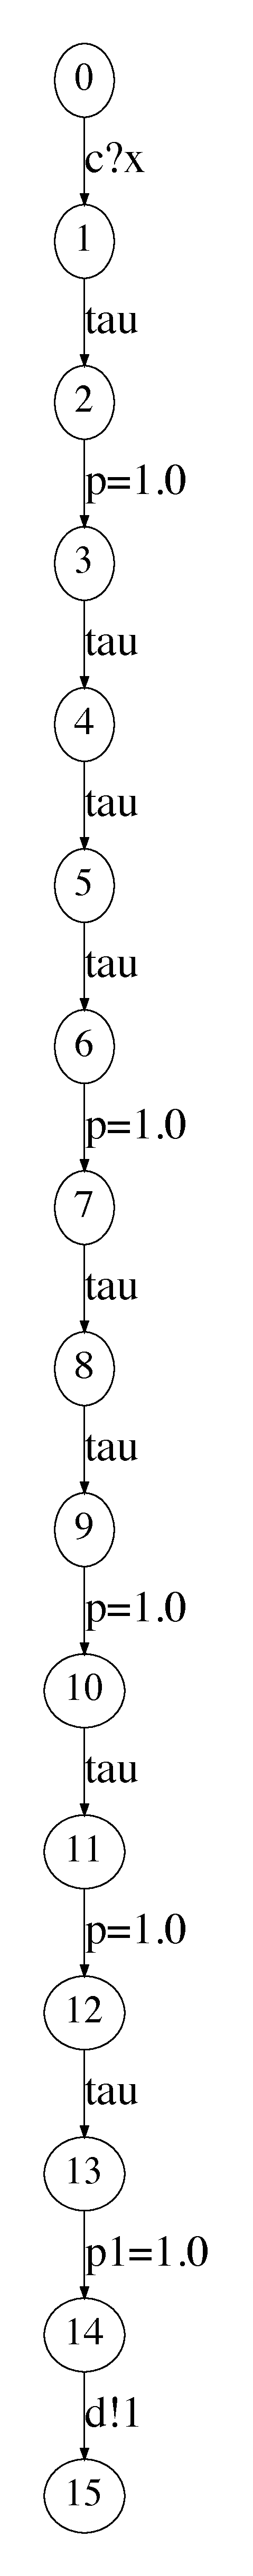
\includegraphics[width=1.75cm]{images/Sdc-1.pdf}}
%   \centerline{\texttt{(a)$Sdc$(x=1)}}
% %   \label{fig:sdc-1}
% \end{minipage}
% \hfill
% \hspace{0.2cm}
% \begin{minipage}{0.1\linewidth}
%   \centerline{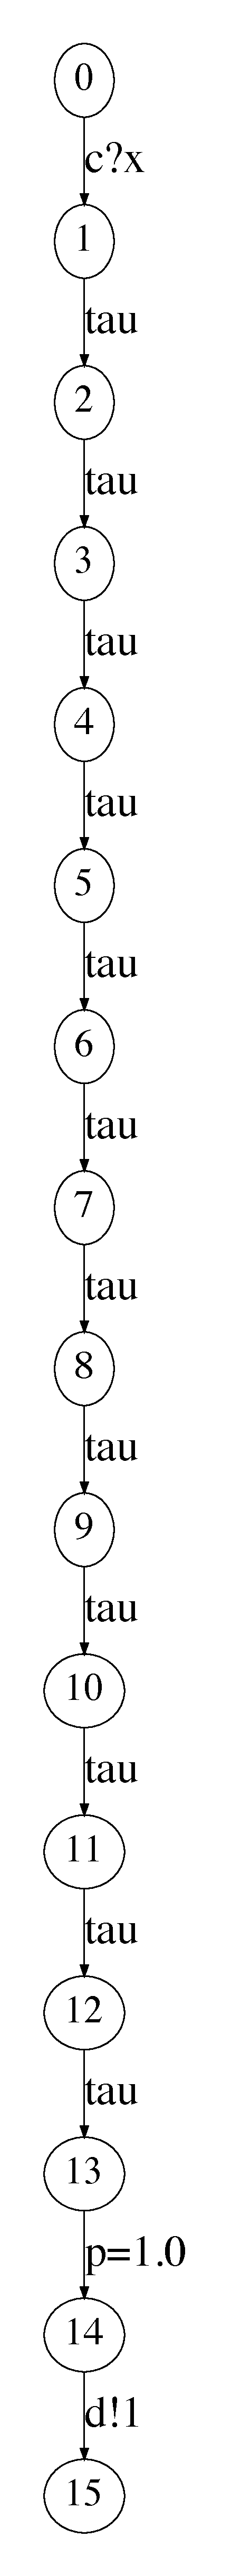
\includegraphics[width=1.6cm]{images/Sdc-spec-1.pdf}}
%   \centerline{\texttt{(b)$Sdc_{spec}$(x=1)}}
% %   \label{fig:sdc-spec-1}
% \end{minipage}
% \hfill
% \begin{minipage}{0.1\linewidth}
%   \centerline{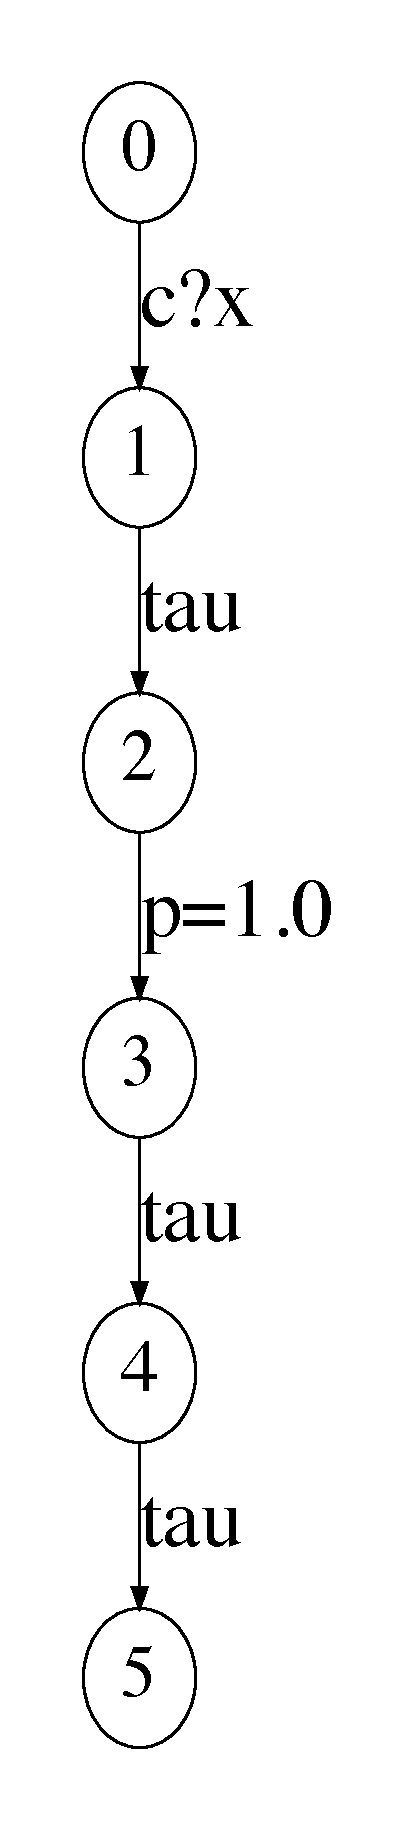
\includegraphics[width=1.6cm]{images/Sdc-2.pdf}}
%   \centerline{\texttt{(c)$Sdc$(x=5)}}
% %   \label{fig:sdc-2}
% \end{minipage}
% \hfill
% \begin{minipage}{0.1\linewidth}
%   \centerline{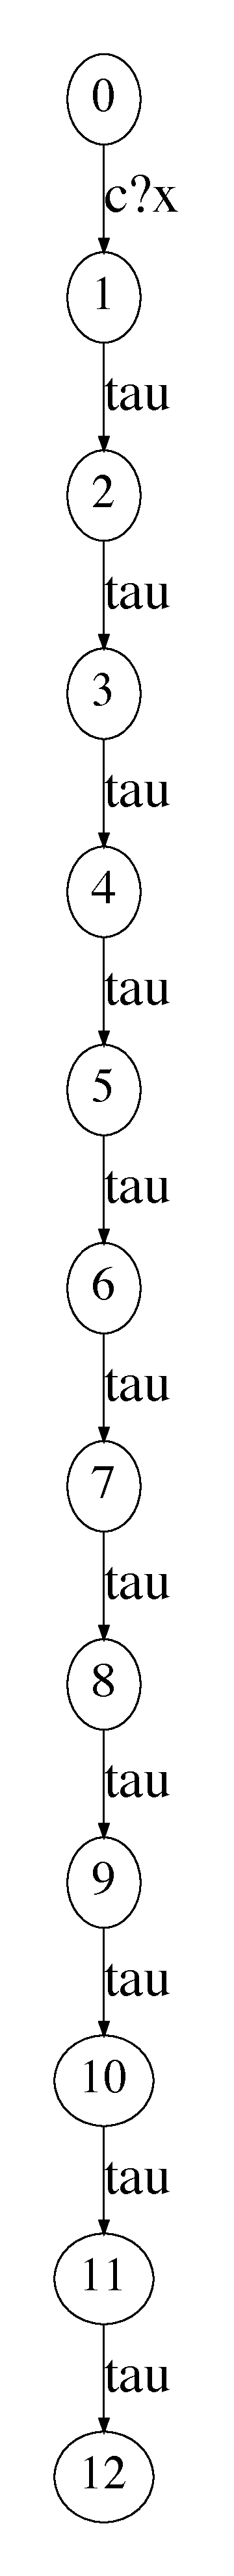
\includegraphics[width=1.35cm]{images/Sdc-spec-2.pdf}}
%   \centerline{\texttt{(d)$Sdc_{spec}$(x=5)}}
% %   \label{fig:sdc-spec-2}
% \end{minipage}
% \hfill
% \hspace{1cm}
% \begin{minipage}{0.2\linewidth}
%   \centerline{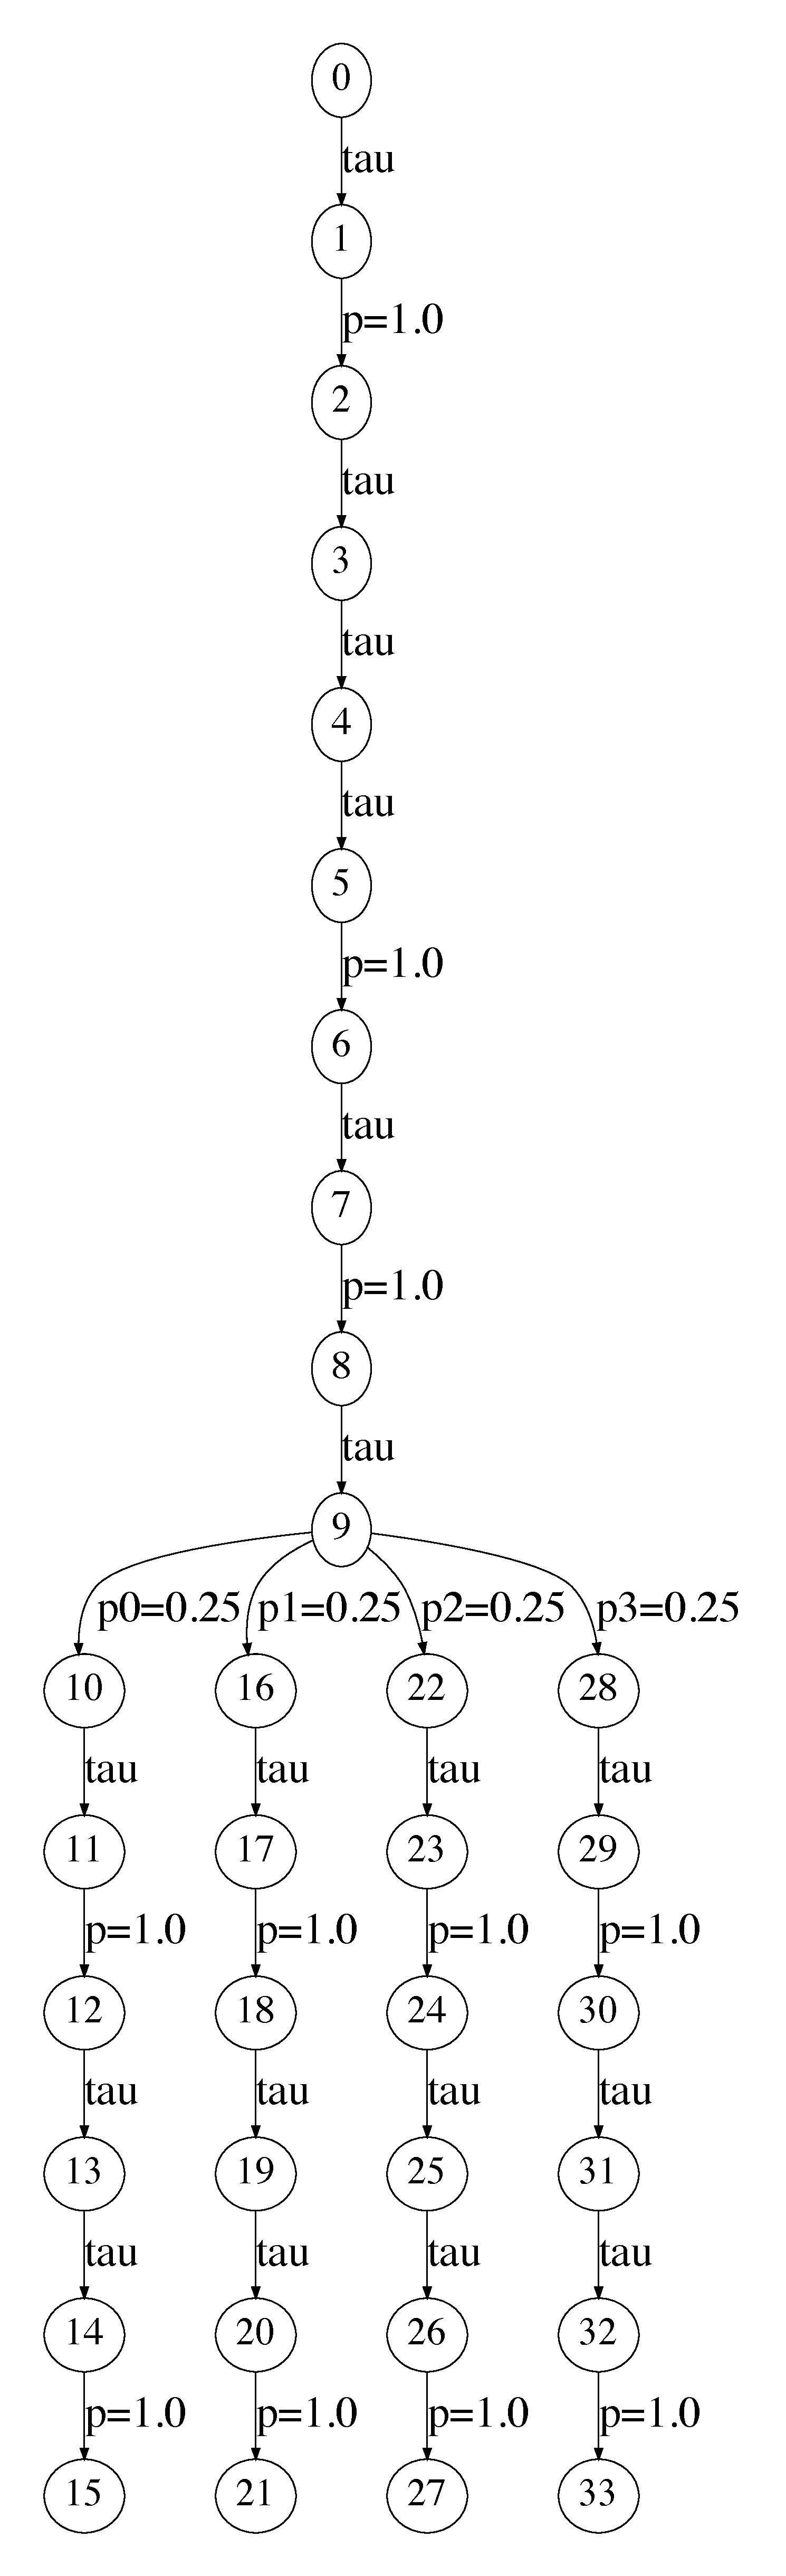
\includegraphics[width=5.4cm]{images/Tele.pdf}}
%   \centerline{\texttt{(e)$Tele$($q_1$=$|1\rangle$)}}
% %   \label{fig:tele}
% \end{minipage}
% \hfill
% \hspace{0.2cm}
% \begin{minipage}{0.1\linewidth}
%   \centerline{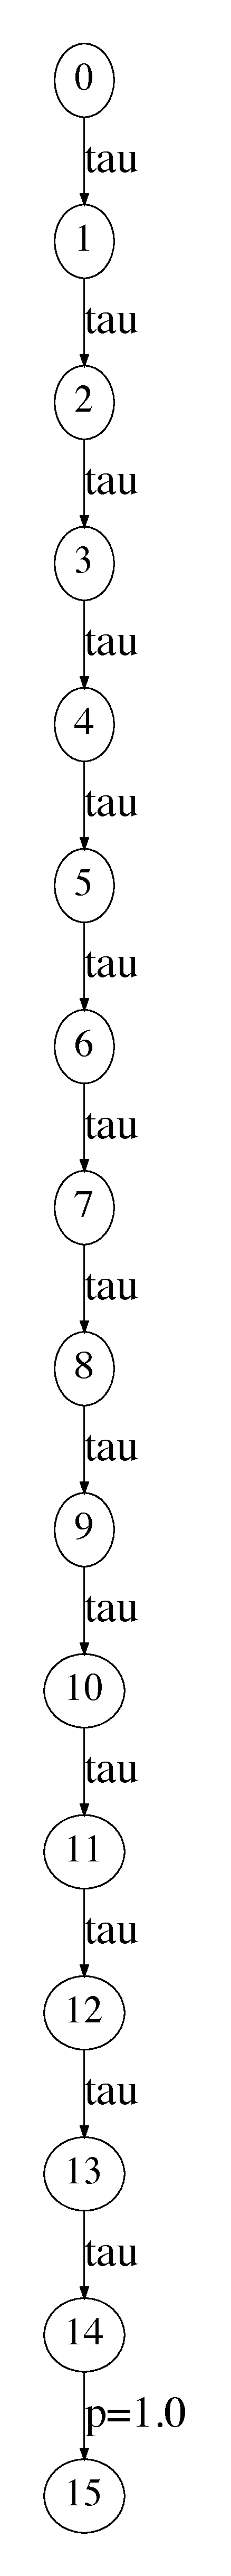
\includegraphics[width=1.6cm]{images/Tele-spec.pdf}}
%   \centerline{\texttt{(f)$Tele_{spec}$($q_1$=$|1\rangle$)}}
% %   \label{fig:tele-spec}
% \end{minipage}
% \caption{Generated pLTSs. $Sdc$ is super-dense coding protocol. $Sdc_{spec}$ is the specification of super-dense coding protocol. $Tele$ is teleportation protocol. $Tele_{spec}$ is the specification of teleportation protocol.}
% \label{fig:sdc+tele}
% \end{figure}
% } %endof leaveout 954

\section{Examples}
\label{sec:examples}
\subsection{Super-dense Coding Protocol}\label{sec:sdc}
% We formalise the super-dense coding protocol. Our formalisation follows \cite{FDY14} to illustrate the use of our tool, where a manual analysis of the protocol is provided. Now we perform automatic verification via the ground bisimulation checker.
% More examples are given in Appendix~\ref{sec:examples}.

Super-dense coding is proposed by Bennett and Wiesner in 1992~\cite{BW92}. It is a quantum communication protocol allowing two classical bits to be encoded in one qubit during a transmission, so it needs only one quantum channel. Such advantage is based on the use of a maximally
entangled state, EPR state. An EPR state can be transformed into all the four kinds of EPR states through a 1-qubit operation, and these EPR states are mutually orthogonal. 
\paragraph{Protocol.}
We suppose the sender and the receiver of the communication are $Alice$ and $Bob$, then the protocol goes as follows:
\begin{enumerate}
    \item $Alice$ and $Bob$ prepare an EPR state $|\beta_{00}\rangle_{q_1,q_2}$ together. Then they share the qubits, $Alice$ holding $q_1$ and $Bob$ holding $q_2$.
    \item If $Alice$ wants to send value $x\in \{0,1,2,3\}$, she applies the corresponding Pauli operation $\sigma^{x}$ on her qubit $q_1$.
    \item $Alice$ sends the qubit $q_1$ to $Bob$.
    \item $Bob$ applies a controlled-not operation on $q_1,q_2$ and a Hadamard operation on $q_1$ to remove the entanglement.
    \item $Bob$ measures $q_1$ and $q_2$ to get the value $x$.
\end{enumerate}
After the execution of the protocol above, $Bob$ gets the value $x$ which $Alice$ wants to send. Note that $x$ could be represented in a 2-bit string. The protocol exactly transmits two classical bits of information by sending one qubit from $Alice$ to $Bob$.
\paragraph{Implementation.}
The modeling of super-dense coding protocol in qCCS follows \cite{FDY14}:
\begin{flalign*}
    Alice \overset{def}{=}& \underline{c}_{A}?q_1.\sum_{0\leq  i\leq 3}(\textbf{if}\ x=i\ \textbf{then}\ \sigma^{i}[q_1].\underline{e}!q_1.\textbf{nil});\\
    Bob \overset{def}{=}& \underline{c}_{B}?q_2.\underline{e}?q_1.CN[q_1,q_2].H[q_1].M[q_1,q_2;x].d!x.\textbf{nil};\\
    EPR \overset{def}{=}& Set^{\Psi}[q_1,q_2].\underline{c}_{B}!q_2.\underline{e}_{A}!q_1.\textbf{nil};\\
    Sdc \overset{def}{=}& c?x.(Alice||Bob||EPR)\setminus \{\underline{c}_{A},\underline{c}_{B},\underline{e}\}
\end{flalign*}
where $CN$ is the controlled-not operation and $H$ is the Hadamard operation, $Set^{\Psi}$ is the operation transforming all the inputs into an EPR state $|\beta_{00}\rangle=(|00\rangle+|11\rangle)/\sqrt{2}$, its operation elements are $\{|\beta_{00}\rangle\langle 00|,|\beta_{00}\rangle\langle 01|,|\beta_{00}\rangle\langle 10|,|\beta_{00}\rangle\langle 11|\}$, and $\sigma^{i}$ are Pauli operators where $\sigma^{0}=I,\sigma^{1}=X,\sigma^{2}=Z,\sigma^{3}=Y$. The element set of measurement \textit{M} is $\{|00\rangle\langle 00|,|01\rangle\langle 01|,|10\rangle\langle 10|,|11\rangle\langle 11|\}$.
\paragraph{Specification.}
The specification of the protocol asks the process to return 2 qubit according to the value of classical bits it received. So it can be defined as:
\begin{flalign*}
    % Sdc_{spec} \overset{def}{=}& c?x.\tau^{11}.\sum_{i=0}^{3}(\textbf{if}\ x=i\ \textbf{then}\ Set^{i}[q_1,q_2].d!x.\textbf{nil})
    Sdc_{spec} \overset{def}{=}& c?x.\sum_{i=0}^{3}(\textbf{if}\ x=i\ \textbf{then}\ Set^{i}[q_1,q_2].d!x.\textbf{nil})
\end{flalign*}
where $Set^{i}$ is the operation of transforming the current state into the state decided by the value of $i$ like $Set^{\Psi}$.
% Here we have inserted some harmless $\tau$-transitions ($\tau^{11}$ stands for a series of $11$ $\tau$-transitions) because in ground bisimulations $\tau$-actions are not abstracted away. 
\paragraph{Input.}
Associated with the specification $Sdc$ are the following variables and operators that need to be declared.
\begin{itemize}
    \item The classical bit is named $x$. It stores the value $Alice$ wants to send. We test the program with different values of $x$.
    \item The qubits are declared as a vector $|q_1,q_2\rangle$. They are used for generating the EPR state here. Without loss of generality, we set them to be $|00\rangle$.
    \item The operation of transforming $|00\rangle$ into the EPR state is defined as $Set^{\Psi}$. 
    \item The controlled-not operation is defined as $CN$.
    \item The Hadamard operation is defined as $H$.
    \item The Pauli operations are defined as $\sigma^0,\sigma^1,\sigma^2$ and $\sigma^3$.
    \item The measurement is defined as $M$ with its operation elements.
\end{itemize}

For the specification $Sdc_{spec}$, we declare the following set of variables and operators.
\begin{itemize}
    \item The classical bit named $x$ is still required to store the value $Alice$ wants to send.
    \item The qubits are declared as a vector $|q_1,q_2\rangle$. We set them to be $|00\rangle$.
    \item The operation of transforming an arbitrary state into $|00\rangle$ (resp. $|01\rangle$, $|10\rangle$, $|11\rangle$) is defined as $Set^{0}$ (resp. $Set^{1}$, $Set^{2}$, $Set^{3}$).
\end{itemize}
%\subparagraph*{Generated pLTSs.}
%The generated pLTSs of the super-dense coding example is illustrated in Figure~\ref{fig:sdc+tele}(a)-Figure~\ref{fig:sdc+tele}(d). If $x=1$, the length of the paths from both sides are 15. However, if $x=5$, the length of the paths from both sides are different.

We see from the first two lines of Table~\ref{tab:weak_result} that not all the inputs can get a positive verification result. In the case $x=1$, we can check that $\langle Sdc,\rho_0\rangle \sim \langle Sdc_{spec},\rho_0\rangle$, where $\rho_0$ is the initial state of the quantum variables. In the case $x=5$, none of the four branches can be chosen, then the tool find that $\langle Sdc,\rho_0\rangle \not\sim \langle Sdc_{spec},\rho_0\rangle$. To correct it, some modifications are needed on both the implementation and the specification.
\paragraph{Improved Super-dense Coding Protocol.}
We improve the above qCCS programs by considering the case $i\neq 1,2,3,4$. In such case we send an alarming message and skip all the rest of operations. The new specification $Sdc'$ is defined below:
\begin{flalign*}
    Alice' \overset{def}{=}& \underline{c}_{A}?q_1.(\sum_{0\leq  i\leq 3}(\textbf{if}\ x=i\ \textbf{then}\ \sigma^{i}[q_1].\underline{e}!q_1.\textbf{nil})\ \\
    &\qquad\qquad\qquad +\ \textbf{if not }\bigvee_{0\leq  i\leq 3} x=i\ \textbf{then}\ c_{C}!msg.\textbf{nil});\\
    % Bob' \overset{def}{=}& \underline{c}_{B}?q_2.(\underline{e}?q_1.CN[q_1,q_2].H[q_1].M[q_1,q_2;x].d!x.\textbf{nil}\ +\ c_{C}?msg.\tau^{8}.d!x.\textbf{nil});\\
    Bob' \overset{def}{=}& \underline{c}_{B}?q_2.(\underline{e}?q_1.CN[q_1,q_2].H[q_1].M[q_1,q_2;x].d!x.\textbf{nil}\ +\ c_{C}?msg.d!x.\textbf{nil});\\
    EPR \overset{def}{=}& Set^{\Psi}[q_1,q_2].\underline{c}_{B}!q_2.\underline{c}_{A}!q_1.\textbf{nil};\\
    Sdc' \overset{def}{=}& c?x.(Alice||Bob||EPR)\setminus \{\underline{c}_{A},\underline{c}_{B},c_{C},\underline{e}\}.
\end{flalign*}
We adjust the specification to add a new branch, so as to get $Sdc'_{spec}$:
\begin{flalign*}
    % Sdc'_{spec} \overset{def}{=}& c?x.\tau^{11}.(\sum_{i=0}^{3}(\textbf{if}\ x=i\ \textbf{then}\ Set^{i}[q_1,q_2].d!x.\textbf{nil})\\
    % &\ +\ \textbf{if}\ \neg\bigvee_{0\leq  i\leq 3} x=i\  \textbf{then}\ Set^{\Psi}[q_1,q_2].d!x.\textbf{nil}).
    Sdc'_{spec} \overset{def}{=}& c?x.(\sum_{i=0}^{3}(\textbf{if}\ x=i\ \textbf{then}\ Set^{i}[q_1,q_2].d!x.\textbf{nil})\\
    &\ +\ \textbf{if not }\bigvee_{0\leq  i\leq 3} x=i\  \textbf{then}\ Set^{\Psi}[q_1,q_2].d!x.\textbf{nil}).
\end{flalign*}

The improved modelling processes are indeed bisimilar, which can be seen in Table~\ref{tab:weak_result}.

\subsection{Quantum Teleportation Protocol}
Quantum teleportation~\cite{BB93} is one of the most important protocols in quantum information theory. It teleports an unknown quantum state by only sending classical information, so it just requires a classical communication channel. It makes use of a maximally entangled state. 
%The post-measurement state can be known from the result of partial measurement for a set of entangled states. 
\paragraph{Protocol.}
Let the sender and the receiver  be $Alice$ and $Bob$, respectively. The quantum teleportation protocol goes as follows:
\begin{enumerate}
    \item $Alice$ and $Bob$ prepare an EPR state $|\beta_{00}\rangle_{q_2,q_3}$ together. Then they share the qubits, $Alice$ holding $q_2$ and $Bob$ holding $q_3$.
    \item To transmit qubit $q_1$, $Alice$ applies a $CN$ operation on $q_1$ and $q_2$ followed by a $H$ operation on $q_1$.
    \item $Alice$ measures $q_1$ and $q_2$ and sends the outcome $x$ to $Bob$.
    \item When $Bob$ receives $x$, he applies the  corresponding $\sigma^{x}$ operation on his qubit $q_3$ to recover the original state of $q_1$.
\end{enumerate}
After the execution, $Bob's$ qubit $q_3$ has the same state as the qubit $q_1$.
\paragraph{Implementation.}
We provide below an implementation of the  quantum teleportation protocol:
\begin{flalign*}
    Alice \overset{def}{=}& \underline{c}_{A}?q_2.CN[q_1,q_2].H[q_1].M[q_1,q_2;x].Set^{\Psi}[q_1,q_2].e!x.\textbf{nil};\\
    Bob \overset{def}{=}& \underline{c}_{B}?q_3.e?x.\sum_{0\leq i\leq 3}(\textbf{if}\ x=i\ \textbf{then}\ \sigma^{i}[q_3].\textbf{nil});\\
    EPR \overset{def}{=}& Set^{\Psi}[q_1,q_2].\underline{c}_{A}!q_2.\underline{c}_{B}!q_3.\textbf{nil};\\
    Tel \overset{def}{=}& (Alice||Bob||EPR)\setminus \{\underline{c}_{A},\underline{c}_{B},e\}
\end{flalign*}
where the operators used here are all already declared before. 
\paragraph{Specification.}
The specification of the protocol can also be described in qCCS. To show the correctness of $Tel$, it suffices to prove that $Tel$ is bisimilar to a swap operation between the first and the thrid qubits, that is $SWAP_{1,3}[q_1,q_3]$. The specification is thus easy.
\begin{flalign*}
    % Tel_{spec} &\overset{def}{=} \tau^{13}.SWAP[q_1,q_3].\textbf{nil}.
    Tel_{spec} &\overset{def}{=}SWAP[q_1,q_3].\textbf{nil}.
\end{flalign*}
\paragraph{Input.}
Some of the operators defined in the input are the same as those  in the super-dense coding example, so we do not repeat them. We need to declare the following variables associated with the implementation.
\begin{itemize}
    \item The classical bits $x$ is declared here  to store the measurement result of qubits $q_1$, $q_2$.
    \item The qubits are declared together as a vector $|q_1,q_2,q_3\rangle$. The first qubit $q_1$ is what $Alice$ wants to teleport.  The values of the last two qubits are arbitrary as they will be transformed into an EPR state later. We set the quantum register to be $|\psi00\rangle$ and test the processes with different values of $|\psi\rangle$.
\end{itemize}
The specification $Tel_{spec} $ declares the same set of variables. And only one operation $SWAP_{1,3}$ is defined in the input.

We see from  Table~\ref{tab:weak_result} that $Tel$ and $Tel_{spec}$ hebave the same with all the three different values of $q_1$.
%\subsection{Quantum Secret Sharing Protocol}
%Quantum Secret Sharing Protocol is first developed by Hillery et al.~\cite{hillery1999quantum}. The problem involves an agent $Alice$ sending information to other two agents $Bob$ and $Charlie$ one of whom is dishonest. It is a classical method which is known as secret sharing that $Alice$ split the information into two parts, then $Bob$ and $Charlie$ need collaboration to get the complete information. It lets the honest one keep the dishonest one from doing damage. A quantum version of it can be realized by a three-qubit maximally entangled state called GHZ state, which has similar property as EPR state. The protocol goes as follows:
%\begin{bracketenumerate}
%    \item $Alice$, $Bob$ and $Charlie$ prepare an GHZ state $(|000\rangle+|111\rangle)/\sqrt{2}_{q_2,q_3,q_4}$ together prior to the following execution. Then they share the qubits, $Alice$ holding $q_2$, $Bob$ holding $q_3$ and $Charlie$ holding $q_4$.
%    \item $Alice$ entangles $q_1$ and $q_2$ applying a $CN$ operation followed by a $H$ operation on $q_1$.
%    \item $Alice$ measures $q_1$ and $q_2$ separately and sends the outcomes $m$ and $n$ to $Charlie$.
%    \item $Bob$ also measures $q_3$ and sends the outcome $o$ to $Charlie$.
%    \item Upon receiving the bits $m$, $n$ and $o$, $Charlie$ retrieves the state through applying Pauli operations $X$ or $Z$ on $q_4$ according to the value of these bits.
%\end{bracketenumerate}
%After the execution, $Charlie's$ qubit $q_4$ has the same state as the qubit $q_1$.
%\subparagraph*{Implementation.}
%The program of quantum teleportation protocol can be encoded in qCCS as follows:
%\begin{flalign*}
%    Alice \overset{def}{=}& \underline{c}_{A}?q2.CN[q_1,q_2].H[q_1].M[q_1;m].M[q_2;n].e!m.f!n.\textbf{nil};\\
%    Bob \overset{def}{=}& \underline{c}_{B}?q_3.H[q_2].M[q_2;o].g!o.\textbf{nil});\\
%    Charlie \overset{def}{=}& \underline{c}_{C}?q_4.e?m.f?n.g?o.\\
%    &\textbf{if}\ o=1\ \textbf{then}\ Z[q_4].\textbf{if}\ m=1\ \textbf{then}\ X[q_4].\textbf{if}\ n=1\ \textbf{then}\ \mathcal{Z}[q_4].\textbf{nil});\\
%    GHZ \overset{def}{=}& Set^{GHZ}[q_2,q_3,q_4].\underline{c}_{A}!q_2.\underline{c}_{B}!q_3.\underline{c}_{C}!q_4.\textbf{nil};\\
%    QSS \overset{def}{=}& (Alice||Bob||Charlie||GHZ)\setminus \{\underline{c}_{A},\underline{c}_{B},\underline{c}_{C},e,f,g\}
%\end{flalign*}
%where the operators used are all already declared before except that $Set^{GHZ}$ is the operation transforming all the inputs into an GHZ state which is similar with $Set^{\Psi}$.
%\subparagraph*{Specification.}
%To show its soundness, we prove that $QSS$ is bisimilar to an swap operation between the first and the fouth qubits, that is $SWAP_{1,4}[q_1,q_4]$. The program can be encoded as follow:
%\begin{flalign*}
%    Spec &\overset{def}{=} \tau^{24}.SWAP[q_1,q_4].\textbf{nil}.
%\end{flalign*}
\subsection{Quantum Secret Sharing Protocol}
Quantum secret sharing protocol is proposed by Hillery et al.~\cite{hillery1999quantum}. The problem involves an agent $Alice$ sending information to other two agents $Bob$ and $Charlie$, one of whom is dishonest. It is a classical method which is known as secret sharing that $Alice$ splits the information into two parts, then $Bob$ and $Charlie$ need to collaborate to get the complete information. The idea is to let the honest one keep the dishonest one from misbehaving. A quantum version of it can be realised by a three-qubit maximally entangled state called GHZ state, which has similar property as EPR states. 
\paragraph{Protocol.}
The protocol goes as follows:
\begin{enumerate}
	\item $Alice$, $Bob$ and $Charlie$ prepare an GHZ state $(|000\rangle+|111\rangle)/\sqrt{2}_{q_2,q_3,q_4}$ together prior to the following execution. Then they share the qubits, $Alice$ holding $q_2$, $Bob$ holding $q_3$ and $Charlie$ holding $q_4$.
	\item $Alice$ entangles $q_1$ and $q_2$ by applying a $CN$ operation followed by a $H$ operation on $q_1$.
	\item $Alice$ measures $q_1$ and $q_2$ separately and sends the outcomes $m$ and $n$ to $Charlie$.
	\item $Bob$ also measures $q_3$ and sends the outcome $o$ to $Charlie$.
	\item Upon receiving the bits $m$, $n$ and $o$, $Charlie$ retrieves the state through applying Pauli operations $X$ or $Z$ on $q_4$ according to the values of these bits.
\end{enumerate}
After the execution, $Charlie's$ qubit $q_4$ has the same state as the qubit $q_1$.
\paragraph{Implementation.}
The quantum secret sharing protocol can be encoded in qCCS as follows:
\begin{flalign*}
Alice \overset{def}{=}& \underline{c}_{A}?q_2.CN[q_1,q_2].H[q_1].M[q_1;m].M[q_2;n].e!m.f!n.\textbf{nil};\\
Bob \overset{def}{=}& \underline{c}_{B}?q_3.H[q_3].M[q_3;o].g!o.\textbf{nil};\\
Charlie \overset{def}{=}& \underline{c}_{C}?q_4.e?m.f?n.g?o.\\
&\textbf{if}\ o=1\ \textbf{then}\ Z[q_4].\textbf{if}\ m=1\ \textbf{then}\ X[q_4].\textbf{if}\ n=1\ \textbf{then}\ Z[q_4].\textbf{nil};\\
GHZ \overset{def}{=}& Set^{GHZ}[q_2,q_3,q_4].\underline{c}_{A}!q_2.\underline{c}_{B}!q_3.\underline{c}_{C}!q_4.\textbf{nil};\\
QSS \overset{def}{=}& (Alice||Bob||Charlie||GHZ)\setminus \{\underline{c}_{A},\underline{c}_{B},\underline{c}_{C},e,f,g\}
\end{flalign*}
where the operators used are all already declared before except that $Set^{GHZ}$ is the operation transforming all the input into a GHZ state.
\paragraph{Specification.}
To show the above implementation is correct, we prove that $QSS$ is bisimilar to a swap operation between the first and the fouth qubits, that is $SWAP_{1,4}[q_1,q_4]$. The specification can be written as follow:
\begin{flalign*}
% QSS_{spec} &\overset{def}{=} \tau^{24}.SWAP[q_1,q_4].\textbf{nil}.
QSS_{spec} &\overset{def}{=}SWAP[q_1,q_4].\textbf{nil}.
\end{flalign*}

%We will investigate this relaxation and  weak ground bisimulations in the future. 
\paragraph{Input.}
In the input of the implementation, we also need to define the Clifford operations and Pauli operations presented before. Other variables and operations are declared as follows.
\begin{itemize}
    \item The classical bits $m$, $n$ and $o$ are declared to store the measurement result of qubits $q_1$, $q_2$ and $q_3$.
    \item The qubits are declared together as a vector $|q_1,q_2,q_3,q_4\rangle$. Similar to the teleportation example, the values of the last three qubits are arbitrary as they will be transformed into a GHZ state later. And the first qubit $q_1$ will be set to several different values to test the implementation.
    \item The operation of transforming an arbitrary state into the GHZ state is defined as $Set^{GHZ}$.
\end{itemize}
The specification process declares the same set of variables. The only operation required is defined as $SWAP_{1,4}$.

We can see from Table~\ref{tab:weak_result} that the implementation behaves the same as the specification for all the three different values of $q_1$.

\subsection{B92 Protocol}
As a simplified version of BB84 protocol, B92 protocol proposed by Bennett~\cite{B92} uses only two kinds of non-orthogonal quantum states such as $|0\rangle$ and $|+\rangle$. It makes the key undetermined during the transmission until $Bob$ finally measures the qubits to prevent the eavesdropper. Such approach bases on the fact that the result of measuring a qubit is nondeterministic if improper basis is chosen.

\paragraph{Protocol.}
Similar to BB84 protocol, let $Alice$ send a sequence of qubits $\tilde{q}$ with size $n$ to $Bob$, the protocol goes as follows:
\begin{enumerate}
    \item $Alice$ randomly generates a sequence of bits $\tilde{B_{a}}$ using her qubits $\tilde{q}$.
    \item $Alice$ chooses a random bits string encoding each data bit as $|0\rangle$ if the corresponding bit in $\tilde{B_{a}}$ is 0, $|+\rangle$ if it is 1.
    \item $Alice$ sends the resulting state to $Bob$.
    \item $Bob$ randomly generates a sequence of $\tilde{B_{b}}$ using his qubits $\tilde{q}'$.
    \item $Bob$ measures the $i$th qubits of $\tilde{q}$ he received from $Alice$ according to the basis according to the $i$th bit of $\tilde{B_{b}}$, $\{|0\rangle, |1\rangle\}$ if it is 0 and $\{|+\rangle, |-\rangle\}$ if it is 1, respectively.
    \item $Bob$ announces the measurement results $\tilde{K_{b}}$ but keeps the measurements he decided.
    \item $Alice$ and $Bob$ keep only those bit pairs from $\tilde{B_{a}}$ and $\tilde{B_{b}}$ for which the result of the measurement (recorded in $\tilde{K_{b}}$) is 1.
\end{enumerate}
As the result still have the probability to be 0 when $Bob$ chooses the improper basis, even if $Alice$ and $Bob$ repeat the protocol with the same bit sequence, they may get different bit pairs.
\paragraph{Implementation.}
Here we give an implementation of the protocol:
\begin{flalign*}
Alice \overset{def}{=}& Ran[q_1;B_{a}].Set_{B_{a}}[q_1].\underline{A2B}!q_1.b2a?K_{b}.\\ 
&\qquad\qquad\qquad(\textbf{if}\ K_{b}=1\ \textbf{then}\ key_{a}!B_{a}.\textbf{nil} + \textbf{if}\ K_{b}=0\ \textbf{then}\ key_{a}!\epsilon.\textbf{nil});\\
Bob \overset{def}{=}& \underline{A2B}?q_1.Ran[q_2;B_{b}].M_{B_{b}}[q_1;K_{b}].b2a!K_{b}.\\
&\qquad\qquad\qquad(\textbf{if}\ K_{b}=1\ \textbf{then}\ key_{b}!B_{b}.\textbf{nil} + \textbf{if}\ K_{b}=0\ \textbf{then}\ key_{b}!\epsilon.\textbf{nil});\\
B92 \overset{def}{=}& (Alice||Bob)\setminus\{a2b,b2a,\underline{A2B}\}
\end{flalign*}
where the operators and special functions have already declared before.
\paragraph{Specification.}
Note that the bit pair are kept only if they satisfy $B_{b}=1-B_{a}$. And we use a $Ran$ to present the nondeterministic result from $Bob$. The specification of the implementation can be written as follows:
\begin{flalign*}
B92_{spec} \overset{def}{=}& Ran[q_1;B_{a}].Ran[q_2;B_{b}].Ran[q_2;K_{b}].\\
&\qquad (\textbf{if}\ B_{a}=B_{b}\ \textbf{then}\ (key_{a}!\epsilon.\textbf{nil}||key_{b}!\epsilon.\textbf{nil})\\
&\qquad + \textbf{if}\ \textbf{not}\ B_{a}=B_{b}\ \textbf{then} (\textbf{if}\ K_{b}=1\ \textbf{then}\ (key_{a}!B_{a}.\textbf{nil}||key_{b}!B_{b}.\textbf{nil})\\
&\qquad\qquad\qquad\qquad\qquad\qquad + \textbf{if}\ K_{b}=0\ \textbf{then}\ (key_{a}!\epsilon.\textbf{nil}||key_{b}!\epsilon.\textbf{nil}))).
\end{flalign*}
\paragraph{Input.}
The implementation of $B92$ need similar operators and functions used in $BB84$ example and need less inputs.
\begin{itemize}
    \item The classical bits are named $B_{a}$ for $Alice$ and $B_{b}$ for $Bob$.
    \item The qubits $|q_1, q_2\rangle$ are set $|00\rangle$ here. $q_2$ is used for generating random number.
\end{itemize}
\subsection{E91 Protocol}
E91 protocol is proposed by Ekert~\cite{E91}, it uses the entanglement property of the quantum states for key distribution. The security of the key is ensured by the property that $Alice$ and $Bob$ get the nondeterministic result through the measurement but the results from both sides are always the same. Furthermore, they can select a subset of the EPR pairs for testing if they violate the Bell's inequality.
\paragraph{Protocol.}
We suppose that $Alice$ is the sender, $Bob$ is the receiver, and there is someone trustworthy to generate the EPR pairs for them. The protocol goes as follows:
\begin{enumerate}
    \item $Alice$ and $Bob$ prepare several EPR states $\tilde{|\beta_{00}\rangle}_{\tilde{q_1},\tilde{q_2}}$ together. Then they share the qubits $\tilde{q_1}$, $\tilde{q_2}$.
    \item When they want to distribute keys, $Alice$ randomly generates a sequence of bits $\tilde{B_{a}}$.
    \item $Alice$ measures the $i$th qubit of $\tilde{q}$ she kept according to the $i$th bit if $\tilde{B_{a}}$. Respectively, the basis is $\{|0\rangle,|1\rangle\}$ if it is 0 and $\{|+\rangle,|-\rangle\}$ if it is 1.
    \item $Bob$ randomly generates a sequence if bits $\tilde{B_{b}}$ and measures the qubits in the same approach.
    \item $Alice$ and $Bob$ announce the $\tilde{B_{a}}$ and $\tilde{B_{b}}$ and keep the qubit if corresponding bit in $\tilde{B_{a}}$, $\tilde{B_{b}}$ are equal. And they test the rest part to see if they violate the Bell's inequality.
\end{enumerate}
\paragraph{Implementation.}
We implement the case that $Alice$ and $Bob$ transmit one data bit through one EPR pair.
\begin{flalign*}
    Alice \overset{def}{=}& \underline{c}_{A}?q_1.Ran[q_3;B_{a}].M_{B_{a}}[q_1;K_{a}].a2b!B_{a}.b2a?B_{b}.key_{a}!cmp(K_{a},B_{a},B_{b}).\textbf{nil};\\
    Bob \overset{def}{=}& \underline{c}_{B}?q_2.Ran[q_4;B_{b}].M_{B_{b}}[q_2;K_{b}].a2b?B_{a}.b2a!B_{b}.key_{b}!cmp(K_{b},B_{b},B_{a}).\textbf{nil};\\
    EPR \overset{def}{=}& Set^{\Psi}[q_1,q_2].\underline{c}_{A}!q_1.\underline{c}_{B}!q_2.\textbf{nil};\\
    E91 \overset{def}{=}& (Alice||Bob||EPR)\setminus \{a2b,b2a,\underline{c}_{A},\underline{c}_{B}\}
\end{flalign*}
where there are some operators and functions already declared before.
\paragraph{Specification.}
The specification is similar to that defined for BB84 protocol:
\begin{flalign*}
E91_{spec} \overset{def}{=}& Ran[q_3;B_{a}].Ran[q_1;K_{a}].Ran[q_4;B_{b}].\\
&\qquad\qquad.(key_{a}!cmp(K_{a},B_{a},B_{b}).\textbf{nil}||key_{b}!cmp(K_{a},B_{a},B_{b}).\textbf{nil}).
\end{flalign*}
\paragraph{Input.}
The implementation of E91 protocol uses more qubits than the protocols before for generating the EPR pairs.
\begin{itemize}
    \item The classical bits are named $B_{a}$, $K_{a}$ for $Alice$ and $B_{b}$, $K_{b}$ for $Bob$.
    \item The qubits $|q_1,q_2\rangle$ is used for preparing EPR pair, they can be initialized as $|00\rangle$. The qubits $|q_3,q_4\rangle$ is used for randomly generation the value of $B_{a}$ and $B_{b}$, they can also be initialized as $|00\rangle$.
\end{itemize}
\section{Matrix Representation of the Operators}\label{sec:appc}
We have frequently used the Hadamard operator, the controlled-not operator and the Pauli operators in our examples. Their matrix representations are listed below.

$$H = 
\begin{bmatrix}
   \frac{1}{\sqrt{2}} & \frac{1}{\sqrt{2}}\\
   \frac{1}{\sqrt{2}} & -\frac{1}{\sqrt{2}}
\end{bmatrix}
\hspace{5em}
CN = 
\begin{bmatrix}
   1 & 0 & 0 & 0\\
   0 & 1 & 0 & 0\\
   0 & 0 & 0 & 1\\
   0 & 0 & 1 & 0
\end{bmatrix}
$$
$$X= 
\begin{bmatrix}
   0 & 1\\
   1 & 0
\end{bmatrix}
\hspace{5em}
Y = 
\begin{bmatrix}
   0 & -i\\
   i & 0
\end{bmatrix}
\hspace{5em}
Z = 
\begin{bmatrix}
   1 & 0\\
   0 & -1
\end{bmatrix}
$$
The quantum operations  $Set^{\Psi}$, $Set^{GHZ}$, $Set^{i}$ are defined using the operator-sum representation~\cite{NC00} with a set of Kraus operators.
\begin{flalign*}
Set^{\Psi}:\quad&
\{\frac{|00\rangle+|11\rangle}{\sqrt{2}}\langle00|,\  \frac{|00\rangle+|11\rangle}{\sqrt{2}}\langle01|,\ \frac{|00\rangle+|11\rangle}{\sqrt{2}}\langle10|,\ \frac{|00\rangle+|11\rangle}{\sqrt{2}}\langle11|\}
\end{flalign*}
\begin{flalign*}
Set^{GHZ}:\quad&
\{\frac{|000\rangle+|111\rangle}{\sqrt{2}}\langle000|,\  \frac{|000\rangle+|111\rangle}{\sqrt{2}}\langle001|,\ \frac{|000\rangle+|111\rangle}{\sqrt{2}}\langle010|,\\
&\frac{|000\rangle+|111\rangle}{\sqrt{2}}\langle011|,\ \frac{|000\rangle+|111\rangle}{\sqrt{2}}\langle100|,\ \frac{|000\rangle+|111\rangle}{\sqrt{2}}\langle101|,\\
&\frac{|000\rangle+|111\rangle}{\sqrt{2}}\langle110|,\ \frac{|000\rangle+|111\rangle}{\sqrt{2}}\langle111|\}
\end{flalign*}
\begin{flalign*}
Set^{0}:
\{|00\rangle\langle00|,|00\rangle\langle01|,|00\rangle\langle10|,|00\rangle\langle11|\}\quad
Set^{1}:
\{|01\rangle\langle00|,|01\rangle\langle01|,|01\rangle\langle10|,|01\rangle\langle11|\}
\end{flalign*}
\begin{flalign*}
Set^{2}:
\{|10\rangle\langle00|,|10\rangle\langle01|,|10\rangle\langle10|,|10\rangle\langle11|\}\quad
Set^{3}:
\{|11\rangle\langle00|,|11\rangle\langle01|,|11\rangle\langle10|,|11\rangle\langle11|\}
\end{flalign*}




\end{document}
